
% Default to the notebook output style

    


% Inherit from the specified cell style.




    
\documentclass[11pt]{article}

    
    
    \usepackage[T1]{fontenc}
    % Nicer default font (+ math font) than Computer Modern for most use cases
    \usepackage{mathpazo}

    % Basic figure setup, for now with no caption control since it's done
    % automatically by Pandoc (which extracts ![](path) syntax from Markdown).
    \usepackage{graphicx}
    % We will generate all images so they have a width \maxwidth. This means
    % that they will get their normal width if they fit onto the page, but
    % are scaled down if they would overflow the margins.
    \makeatletter
    \def\maxwidth{\ifdim\Gin@nat@width>\linewidth\linewidth
    \else\Gin@nat@width\fi}
    \makeatother
    \let\Oldincludegraphics\includegraphics
    % Set max figure width to be 80% of text width, for now hardcoded.
    \renewcommand{\includegraphics}[1]{\Oldincludegraphics[width=.8\maxwidth]{#1}}
    % Ensure that by default, figures have no caption (until we provide a
    % proper Figure object with a Caption API and a way to capture that
    % in the conversion process - todo).
    \usepackage{caption}
    \DeclareCaptionLabelFormat{nolabel}{}
    \captionsetup{labelformat=nolabel}

    \usepackage{adjustbox} % Used to constrain images to a maximum size 
    \usepackage{xcolor} % Allow colors to be defined
    \usepackage{enumerate} % Needed for markdown enumerations to work
    \usepackage{geometry} % Used to adjust the document margins
    \usepackage{amsmath} % Equations
    \usepackage{amssymb} % Equations
    \usepackage{textcomp} % defines textquotesingle
    % Hack from http://tex.stackexchange.com/a/47451/13684:
    \AtBeginDocument{%
        \def\PYZsq{\textquotesingle}% Upright quotes in Pygmentized code
    }
    \usepackage{upquote} % Upright quotes for verbatim code
    \usepackage{eurosym} % defines \euro
    \usepackage[mathletters]{ucs} % Extended unicode (utf-8) support
    \usepackage[utf8x]{inputenc} % Allow utf-8 characters in the tex document
    \usepackage{fancyvrb} % verbatim replacement that allows latex
    \usepackage{grffile} % extends the file name processing of package graphics 
                         % to support a larger range 
    % The hyperref package gives us a pdf with properly built
    % internal navigation ('pdf bookmarks' for the table of contents,
    % internal cross-reference links, web links for URLs, etc.)
    \usepackage{hyperref}
    \usepackage{longtable} % longtable support required by pandoc >1.10
    \usepackage{booktabs}  % table support for pandoc > 1.12.2
    \usepackage[inline]{enumitem} % IRkernel/repr support (it uses the enumerate* environment)
    \usepackage[normalem]{ulem} % ulem is needed to support strikethroughs (\sout)
                                % normalem makes italics be italics, not underlines
    

    
    
    % Colors for the hyperref package
    \definecolor{urlcolor}{rgb}{0,.145,.698}
    \definecolor{linkcolor}{rgb}{.71,0.21,0.01}
    \definecolor{citecolor}{rgb}{.12,.54,.11}

    % ANSI colors
    \definecolor{ansi-black}{HTML}{3E424D}
    \definecolor{ansi-black-intense}{HTML}{282C36}
    \definecolor{ansi-red}{HTML}{E75C58}
    \definecolor{ansi-red-intense}{HTML}{B22B31}
    \definecolor{ansi-green}{HTML}{00A250}
    \definecolor{ansi-green-intense}{HTML}{007427}
    \definecolor{ansi-yellow}{HTML}{DDB62B}
    \definecolor{ansi-yellow-intense}{HTML}{B27D12}
    \definecolor{ansi-blue}{HTML}{208FFB}
    \definecolor{ansi-blue-intense}{HTML}{0065CA}
    \definecolor{ansi-magenta}{HTML}{D160C4}
    \definecolor{ansi-magenta-intense}{HTML}{A03196}
    \definecolor{ansi-cyan}{HTML}{60C6C8}
    \definecolor{ansi-cyan-intense}{HTML}{258F8F}
    \definecolor{ansi-white}{HTML}{C5C1B4}
    \definecolor{ansi-white-intense}{HTML}{A1A6B2}

    % commands and environments needed by pandoc snippets
    % extracted from the output of `pandoc -s`
    \providecommand{\tightlist}{%
      \setlength{\itemsep}{0pt}\setlength{\parskip}{0pt}}
    \DefineVerbatimEnvironment{Highlighting}{Verbatim}{commandchars=\\\{\}}
    % Add ',fontsize=\small' for more characters per line
    \newenvironment{Shaded}{}{}
    \newcommand{\KeywordTok}[1]{\textcolor[rgb]{0.00,0.44,0.13}{\textbf{{#1}}}}
    \newcommand{\DataTypeTok}[1]{\textcolor[rgb]{0.56,0.13,0.00}{{#1}}}
    \newcommand{\DecValTok}[1]{\textcolor[rgb]{0.25,0.63,0.44}{{#1}}}
    \newcommand{\BaseNTok}[1]{\textcolor[rgb]{0.25,0.63,0.44}{{#1}}}
    \newcommand{\FloatTok}[1]{\textcolor[rgb]{0.25,0.63,0.44}{{#1}}}
    \newcommand{\CharTok}[1]{\textcolor[rgb]{0.25,0.44,0.63}{{#1}}}
    \newcommand{\StringTok}[1]{\textcolor[rgb]{0.25,0.44,0.63}{{#1}}}
    \newcommand{\CommentTok}[1]{\textcolor[rgb]{0.38,0.63,0.69}{\textit{{#1}}}}
    \newcommand{\OtherTok}[1]{\textcolor[rgb]{0.00,0.44,0.13}{{#1}}}
    \newcommand{\AlertTok}[1]{\textcolor[rgb]{1.00,0.00,0.00}{\textbf{{#1}}}}
    \newcommand{\FunctionTok}[1]{\textcolor[rgb]{0.02,0.16,0.49}{{#1}}}
    \newcommand{\RegionMarkerTok}[1]{{#1}}
    \newcommand{\ErrorTok}[1]{\textcolor[rgb]{1.00,0.00,0.00}{\textbf{{#1}}}}
    \newcommand{\NormalTok}[1]{{#1}}
    
    % Additional commands for more recent versions of Pandoc
    \newcommand{\ConstantTok}[1]{\textcolor[rgb]{0.53,0.00,0.00}{{#1}}}
    \newcommand{\SpecialCharTok}[1]{\textcolor[rgb]{0.25,0.44,0.63}{{#1}}}
    \newcommand{\VerbatimStringTok}[1]{\textcolor[rgb]{0.25,0.44,0.63}{{#1}}}
    \newcommand{\SpecialStringTok}[1]{\textcolor[rgb]{0.73,0.40,0.53}{{#1}}}
    \newcommand{\ImportTok}[1]{{#1}}
    \newcommand{\DocumentationTok}[1]{\textcolor[rgb]{0.73,0.13,0.13}{\textit{{#1}}}}
    \newcommand{\AnnotationTok}[1]{\textcolor[rgb]{0.38,0.63,0.69}{\textbf{\textit{{#1}}}}}
    \newcommand{\CommentVarTok}[1]{\textcolor[rgb]{0.38,0.63,0.69}{\textbf{\textit{{#1}}}}}
    \newcommand{\VariableTok}[1]{\textcolor[rgb]{0.10,0.09,0.49}{{#1}}}
    \newcommand{\ControlFlowTok}[1]{\textcolor[rgb]{0.00,0.44,0.13}{\textbf{{#1}}}}
    \newcommand{\OperatorTok}[1]{\textcolor[rgb]{0.40,0.40,0.40}{{#1}}}
    \newcommand{\BuiltInTok}[1]{{#1}}
    \newcommand{\ExtensionTok}[1]{{#1}}
    \newcommand{\PreprocessorTok}[1]{\textcolor[rgb]{0.74,0.48,0.00}{{#1}}}
    \newcommand{\AttributeTok}[1]{\textcolor[rgb]{0.49,0.56,0.16}{{#1}}}
    \newcommand{\InformationTok}[1]{\textcolor[rgb]{0.38,0.63,0.69}{\textbf{\textit{{#1}}}}}
    \newcommand{\WarningTok}[1]{\textcolor[rgb]{0.38,0.63,0.69}{\textbf{\textit{{#1}}}}}
    
    
    % Define a nice break command that doesn't care if a line doesn't already
    % exist.
    \def\br{\hspace*{\fill} \\* }
    % Math Jax compatability definitions
    \def\gt{>}
    \def\lt{<}
    % Document parameters
    \title{Report}
    
    
    

    % Pygments definitions
    
\makeatletter
\def\PY@reset{\let\PY@it=\relax \let\PY@bf=\relax%
    \let\PY@ul=\relax \let\PY@tc=\relax%
    \let\PY@bc=\relax \let\PY@ff=\relax}
\def\PY@tok#1{\csname PY@tok@#1\endcsname}
\def\PY@toks#1+{\ifx\relax#1\empty\else%
    \PY@tok{#1}\expandafter\PY@toks\fi}
\def\PY@do#1{\PY@bc{\PY@tc{\PY@ul{%
    \PY@it{\PY@bf{\PY@ff{#1}}}}}}}
\def\PY#1#2{\PY@reset\PY@toks#1+\relax+\PY@do{#2}}

\expandafter\def\csname PY@tok@w\endcsname{\def\PY@tc##1{\textcolor[rgb]{0.73,0.73,0.73}{##1}}}
\expandafter\def\csname PY@tok@c\endcsname{\let\PY@it=\textit\def\PY@tc##1{\textcolor[rgb]{0.25,0.50,0.50}{##1}}}
\expandafter\def\csname PY@tok@cp\endcsname{\def\PY@tc##1{\textcolor[rgb]{0.74,0.48,0.00}{##1}}}
\expandafter\def\csname PY@tok@k\endcsname{\let\PY@bf=\textbf\def\PY@tc##1{\textcolor[rgb]{0.00,0.50,0.00}{##1}}}
\expandafter\def\csname PY@tok@kp\endcsname{\def\PY@tc##1{\textcolor[rgb]{0.00,0.50,0.00}{##1}}}
\expandafter\def\csname PY@tok@kt\endcsname{\def\PY@tc##1{\textcolor[rgb]{0.69,0.00,0.25}{##1}}}
\expandafter\def\csname PY@tok@o\endcsname{\def\PY@tc##1{\textcolor[rgb]{0.40,0.40,0.40}{##1}}}
\expandafter\def\csname PY@tok@ow\endcsname{\let\PY@bf=\textbf\def\PY@tc##1{\textcolor[rgb]{0.67,0.13,1.00}{##1}}}
\expandafter\def\csname PY@tok@nb\endcsname{\def\PY@tc##1{\textcolor[rgb]{0.00,0.50,0.00}{##1}}}
\expandafter\def\csname PY@tok@nf\endcsname{\def\PY@tc##1{\textcolor[rgb]{0.00,0.00,1.00}{##1}}}
\expandafter\def\csname PY@tok@nc\endcsname{\let\PY@bf=\textbf\def\PY@tc##1{\textcolor[rgb]{0.00,0.00,1.00}{##1}}}
\expandafter\def\csname PY@tok@nn\endcsname{\let\PY@bf=\textbf\def\PY@tc##1{\textcolor[rgb]{0.00,0.00,1.00}{##1}}}
\expandafter\def\csname PY@tok@ne\endcsname{\let\PY@bf=\textbf\def\PY@tc##1{\textcolor[rgb]{0.82,0.25,0.23}{##1}}}
\expandafter\def\csname PY@tok@nv\endcsname{\def\PY@tc##1{\textcolor[rgb]{0.10,0.09,0.49}{##1}}}
\expandafter\def\csname PY@tok@no\endcsname{\def\PY@tc##1{\textcolor[rgb]{0.53,0.00,0.00}{##1}}}
\expandafter\def\csname PY@tok@nl\endcsname{\def\PY@tc##1{\textcolor[rgb]{0.63,0.63,0.00}{##1}}}
\expandafter\def\csname PY@tok@ni\endcsname{\let\PY@bf=\textbf\def\PY@tc##1{\textcolor[rgb]{0.60,0.60,0.60}{##1}}}
\expandafter\def\csname PY@tok@na\endcsname{\def\PY@tc##1{\textcolor[rgb]{0.49,0.56,0.16}{##1}}}
\expandafter\def\csname PY@tok@nt\endcsname{\let\PY@bf=\textbf\def\PY@tc##1{\textcolor[rgb]{0.00,0.50,0.00}{##1}}}
\expandafter\def\csname PY@tok@nd\endcsname{\def\PY@tc##1{\textcolor[rgb]{0.67,0.13,1.00}{##1}}}
\expandafter\def\csname PY@tok@s\endcsname{\def\PY@tc##1{\textcolor[rgb]{0.73,0.13,0.13}{##1}}}
\expandafter\def\csname PY@tok@sd\endcsname{\let\PY@it=\textit\def\PY@tc##1{\textcolor[rgb]{0.73,0.13,0.13}{##1}}}
\expandafter\def\csname PY@tok@si\endcsname{\let\PY@bf=\textbf\def\PY@tc##1{\textcolor[rgb]{0.73,0.40,0.53}{##1}}}
\expandafter\def\csname PY@tok@se\endcsname{\let\PY@bf=\textbf\def\PY@tc##1{\textcolor[rgb]{0.73,0.40,0.13}{##1}}}
\expandafter\def\csname PY@tok@sr\endcsname{\def\PY@tc##1{\textcolor[rgb]{0.73,0.40,0.53}{##1}}}
\expandafter\def\csname PY@tok@ss\endcsname{\def\PY@tc##1{\textcolor[rgb]{0.10,0.09,0.49}{##1}}}
\expandafter\def\csname PY@tok@sx\endcsname{\def\PY@tc##1{\textcolor[rgb]{0.00,0.50,0.00}{##1}}}
\expandafter\def\csname PY@tok@m\endcsname{\def\PY@tc##1{\textcolor[rgb]{0.40,0.40,0.40}{##1}}}
\expandafter\def\csname PY@tok@gh\endcsname{\let\PY@bf=\textbf\def\PY@tc##1{\textcolor[rgb]{0.00,0.00,0.50}{##1}}}
\expandafter\def\csname PY@tok@gu\endcsname{\let\PY@bf=\textbf\def\PY@tc##1{\textcolor[rgb]{0.50,0.00,0.50}{##1}}}
\expandafter\def\csname PY@tok@gd\endcsname{\def\PY@tc##1{\textcolor[rgb]{0.63,0.00,0.00}{##1}}}
\expandafter\def\csname PY@tok@gi\endcsname{\def\PY@tc##1{\textcolor[rgb]{0.00,0.63,0.00}{##1}}}
\expandafter\def\csname PY@tok@gr\endcsname{\def\PY@tc##1{\textcolor[rgb]{1.00,0.00,0.00}{##1}}}
\expandafter\def\csname PY@tok@ge\endcsname{\let\PY@it=\textit}
\expandafter\def\csname PY@tok@gs\endcsname{\let\PY@bf=\textbf}
\expandafter\def\csname PY@tok@gp\endcsname{\let\PY@bf=\textbf\def\PY@tc##1{\textcolor[rgb]{0.00,0.00,0.50}{##1}}}
\expandafter\def\csname PY@tok@go\endcsname{\def\PY@tc##1{\textcolor[rgb]{0.53,0.53,0.53}{##1}}}
\expandafter\def\csname PY@tok@gt\endcsname{\def\PY@tc##1{\textcolor[rgb]{0.00,0.27,0.87}{##1}}}
\expandafter\def\csname PY@tok@err\endcsname{\def\PY@bc##1{\setlength{\fboxsep}{0pt}\fcolorbox[rgb]{1.00,0.00,0.00}{1,1,1}{\strut ##1}}}
\expandafter\def\csname PY@tok@kc\endcsname{\let\PY@bf=\textbf\def\PY@tc##1{\textcolor[rgb]{0.00,0.50,0.00}{##1}}}
\expandafter\def\csname PY@tok@kd\endcsname{\let\PY@bf=\textbf\def\PY@tc##1{\textcolor[rgb]{0.00,0.50,0.00}{##1}}}
\expandafter\def\csname PY@tok@kn\endcsname{\let\PY@bf=\textbf\def\PY@tc##1{\textcolor[rgb]{0.00,0.50,0.00}{##1}}}
\expandafter\def\csname PY@tok@kr\endcsname{\let\PY@bf=\textbf\def\PY@tc##1{\textcolor[rgb]{0.00,0.50,0.00}{##1}}}
\expandafter\def\csname PY@tok@bp\endcsname{\def\PY@tc##1{\textcolor[rgb]{0.00,0.50,0.00}{##1}}}
\expandafter\def\csname PY@tok@fm\endcsname{\def\PY@tc##1{\textcolor[rgb]{0.00,0.00,1.00}{##1}}}
\expandafter\def\csname PY@tok@vc\endcsname{\def\PY@tc##1{\textcolor[rgb]{0.10,0.09,0.49}{##1}}}
\expandafter\def\csname PY@tok@vg\endcsname{\def\PY@tc##1{\textcolor[rgb]{0.10,0.09,0.49}{##1}}}
\expandafter\def\csname PY@tok@vi\endcsname{\def\PY@tc##1{\textcolor[rgb]{0.10,0.09,0.49}{##1}}}
\expandafter\def\csname PY@tok@vm\endcsname{\def\PY@tc##1{\textcolor[rgb]{0.10,0.09,0.49}{##1}}}
\expandafter\def\csname PY@tok@sa\endcsname{\def\PY@tc##1{\textcolor[rgb]{0.73,0.13,0.13}{##1}}}
\expandafter\def\csname PY@tok@sb\endcsname{\def\PY@tc##1{\textcolor[rgb]{0.73,0.13,0.13}{##1}}}
\expandafter\def\csname PY@tok@sc\endcsname{\def\PY@tc##1{\textcolor[rgb]{0.73,0.13,0.13}{##1}}}
\expandafter\def\csname PY@tok@dl\endcsname{\def\PY@tc##1{\textcolor[rgb]{0.73,0.13,0.13}{##1}}}
\expandafter\def\csname PY@tok@s2\endcsname{\def\PY@tc##1{\textcolor[rgb]{0.73,0.13,0.13}{##1}}}
\expandafter\def\csname PY@tok@sh\endcsname{\def\PY@tc##1{\textcolor[rgb]{0.73,0.13,0.13}{##1}}}
\expandafter\def\csname PY@tok@s1\endcsname{\def\PY@tc##1{\textcolor[rgb]{0.73,0.13,0.13}{##1}}}
\expandafter\def\csname PY@tok@mb\endcsname{\def\PY@tc##1{\textcolor[rgb]{0.40,0.40,0.40}{##1}}}
\expandafter\def\csname PY@tok@mf\endcsname{\def\PY@tc##1{\textcolor[rgb]{0.40,0.40,0.40}{##1}}}
\expandafter\def\csname PY@tok@mh\endcsname{\def\PY@tc##1{\textcolor[rgb]{0.40,0.40,0.40}{##1}}}
\expandafter\def\csname PY@tok@mi\endcsname{\def\PY@tc##1{\textcolor[rgb]{0.40,0.40,0.40}{##1}}}
\expandafter\def\csname PY@tok@il\endcsname{\def\PY@tc##1{\textcolor[rgb]{0.40,0.40,0.40}{##1}}}
\expandafter\def\csname PY@tok@mo\endcsname{\def\PY@tc##1{\textcolor[rgb]{0.40,0.40,0.40}{##1}}}
\expandafter\def\csname PY@tok@ch\endcsname{\let\PY@it=\textit\def\PY@tc##1{\textcolor[rgb]{0.25,0.50,0.50}{##1}}}
\expandafter\def\csname PY@tok@cm\endcsname{\let\PY@it=\textit\def\PY@tc##1{\textcolor[rgb]{0.25,0.50,0.50}{##1}}}
\expandafter\def\csname PY@tok@cpf\endcsname{\let\PY@it=\textit\def\PY@tc##1{\textcolor[rgb]{0.25,0.50,0.50}{##1}}}
\expandafter\def\csname PY@tok@c1\endcsname{\let\PY@it=\textit\def\PY@tc##1{\textcolor[rgb]{0.25,0.50,0.50}{##1}}}
\expandafter\def\csname PY@tok@cs\endcsname{\let\PY@it=\textit\def\PY@tc##1{\textcolor[rgb]{0.25,0.50,0.50}{##1}}}

\def\PYZbs{\char`\\}
\def\PYZus{\char`\_}
\def\PYZob{\char`\{}
\def\PYZcb{\char`\}}
\def\PYZca{\char`\^}
\def\PYZam{\char`\&}
\def\PYZlt{\char`\<}
\def\PYZgt{\char`\>}
\def\PYZsh{\char`\#}
\def\PYZpc{\char`\%}
\def\PYZdl{\char`\$}
\def\PYZhy{\char`\-}
\def\PYZsq{\char`\'}
\def\PYZdq{\char`\"}
\def\PYZti{\char`\~}
% for compatibility with earlier versions
\def\PYZat{@}
\def\PYZlb{[}
\def\PYZrb{]}
\makeatother


    % Exact colors from NB
    \definecolor{incolor}{rgb}{0.0, 0.0, 0.5}
    \definecolor{outcolor}{rgb}{0.545, 0.0, 0.0}



    
    % Prevent overflowing lines due to hard-to-break entities
    \sloppy 
    % Setup hyperref package
    \hypersetup{
      breaklinks=true,  % so long urls are correctly broken across lines
      colorlinks=true,
      urlcolor=urlcolor,
      linkcolor=linkcolor,
      citecolor=citecolor,
      }
    % Slightly bigger margins than the latex defaults
    
    \geometry{verbose,tmargin=1in,bmargin=1in,lmargin=1in,rmargin=1in}
    
    

    \begin{document}
    
    
    \maketitle
    
    

    
    \hypertarget{reproducibility-project-wamda-weighted-alignment-of-sources-for-multi-source-domain-adaptation}{%
\section{Reproducibility Project: WAMDA: Weighted Alignment of Sources
for Multi-source Domain
Adaptation}\label{reproducibility-project-wamda-weighted-alignment-of-sources-for-multi-source-domain-adaptation}}

    \hypertarget{group-10-jiaming-xu-5247578-and-siwei-wang-5239982}{%
\subsubsection{Group 10 Jiaming Xu (5247578) and Siwei Wang
(5239982)}\label{group-10-jiaming-xu-5247578-and-siwei-wang-5239982}}

    \hypertarget{introduction}{%
\subsection{Introduction}\label{introduction}}

One of the learning goals for Deep Learning course is to reproduce a
paper given by the course instructor. This blog gives clear information
about our reproduce work for the paper WAMDA: Weighted Alignment of
Sources for Multi-source Domain Adaptation from Surbhi Aggarwal,
Jogendra Nath Kundu, R. Venkatesh Babu, and Anirban Chakraborty. Our
reproduction is based on the original paper, also some other papers
related to Multi-source Domain Adaptation,and online resources.

The paper presents a novel method for Multi-source Domain Adaptation
named WAMDA which uses multiple sources to train a predictor based on
their internal relevance and their relevance score related to the
target. Our work is to reproduce the proposed approach on only one
dataset \textbf{OfficeHome dataset} and the other two methods (Resnet
and MFSAN for evaluating the effectiveness of the proposed method).

    \hypertarget{model-sturcture}{%
\subsection{Model sturcture}\label{model-sturcture}}

WAMDA is a method that can do effective multi-source domain adaptation
based on the source-target and source-source similarities. The following
gives information about the basic structure.

The proposed algorithm is divided into two parts. The first stage is
\emph{pre-adaptation training} , we can obtain the relevance score,
feature extractor, source classifier, and domain classifier from this
stage. Then, the other stage is \emph{multi-source adaptation training}
, the weighted alignment of domains is performed, classifiers and a
target encoder are learned based on this weighted aligned space. The
basic model structure is shown as follows:
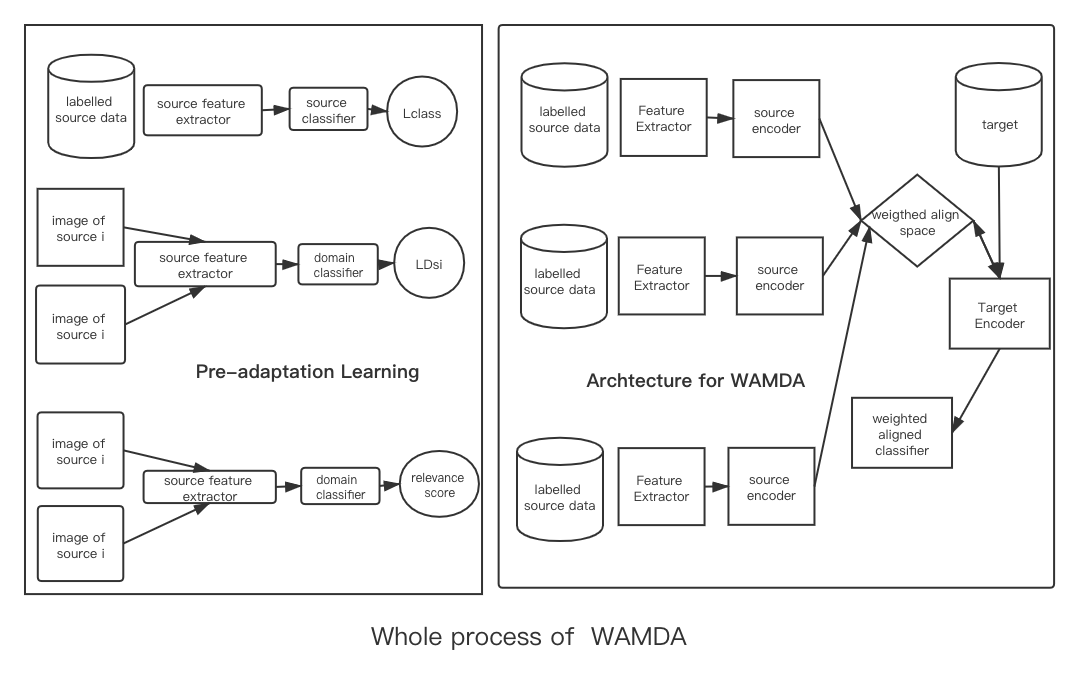
\includegraphics{imgs/process.png}

    \hypertarget{experiment-setup}{%
\subsection{Experiment Setup}\label{experiment-setup}}

The original paper did experiments on three datasets(\emph{Office-31,
Office-Caltech, and Office-Home}). In addition, it uses four types of
baseline(\emph{No Adapt, Single-Source Best, Single-Source Best, and
Multi-Source} to analyze the performance of MSDA methods. For our
experiment, we only did experiment on \emph{office-Home} dataset and
there are only two types of baseline we have implemented: (1) \emph{No
Adapt}: Resnet and the Proposed method (2)\emph{Multi-Source}: MFSAN and
the Proposed method. Last but not the least, the implementation steps
are just the same as the original paper and will be described in the
next section. Due to time limitations, we only have to implement the
first row and the third row of table 5 for \textbf{OfficeHomeDataset}.

    \hypertarget{our-implementaion}{%
\subsection{Our implementaion}\label{our-implementaion}}

All the experiments were done on Google Colab, and the framework we used
is PyTorch. This method is achieved by these steps. First, the dataset
was downloaded and transferred into a certain format. Then,we trained
feature extractors, source classifiers, and a domain classifier based on
the datasets. After that, we extract the relevance scores from the last
step, and the scores will be used in the following steps. We also
trained weighted aligned source encoders, target classifiers, and a
target encoder.

The following libaries are used in onr experiment.

    \begin{Verbatim}[commandchars=\\\{\}]
{\color{incolor}In [{\color{incolor} }]:} \PY{k+kn}{import} \PY{n+nn}{time}
        \PY{k+kn}{import} \PY{n+nn}{copy}
        \PY{k+kn}{import} \PY{n+nn}{torch}
        \PY{k+kn}{import} \PY{n+nn}{numpy} \PY{k}{as} \PY{n+nn}{np}
        \PY{k+kn}{import} \PY{n+nn}{os}
        \PY{k+kn}{from} \PY{n+nn}{tqdm} \PY{k}{import} \PY{n}{tqdm}
        \PY{k+kn}{from} \PY{n+nn}{torch}\PY{n+nn}{.}\PY{n+nn}{utils}\PY{n+nn}{.}\PY{n+nn}{data}\PY{n+nn}{.}\PY{n+nn}{sampler} \PY{k}{import} \PY{n}{SubsetRandomSampler}
        \PY{k+kn}{from} \PY{n+nn}{torchvision} \PY{k}{import} \PY{n}{transforms}
        \PY{k+kn}{import} \PY{n+nn}{torch}\PY{n+nn}{.}\PY{n+nn}{nn} \PY{k}{as} \PY{n+nn}{nn}
        \PY{k+kn}{from} \PY{n+nn}{torchvision} \PY{k}{import} \PY{n}{transforms}
        \PY{k+kn}{from} \PY{n+nn}{torch}\PY{n+nn}{.}\PY{n+nn}{utils}\PY{n+nn}{.}\PY{n+nn}{data} \PY{k}{import} \PY{n}{DataLoader}
        \PY{k+kn}{import} \PY{n+nn}{torch}\PY{n+nn}{.}\PY{n+nn}{optim} \PY{k}{as} \PY{n+nn}{optim}
        \PY{k+kn}{import} \PY{n+nn}{torch}\PY{n+nn}{.}\PY{n+nn}{nn}\PY{n+nn}{.}\PY{n+nn}{functional} \PY{k}{as} \PY{n+nn}{F}
        \PY{k+kn}{from} \PY{n+nn}{torch}\PY{n+nn}{.}\PY{n+nn}{autograd} \PY{k}{import} \PY{n}{Variable}
        \PY{k+kn}{import} \PY{n+nn}{os}
        \PY{k+kn}{from} \PY{n+nn}{torch}\PY{n+nn}{.}\PY{n+nn}{utils}\PY{n+nn}{.}\PY{n+nn}{data} \PY{k}{import} \PY{n}{Dataset}
        \PY{k+kn}{from} \PY{n+nn}{torchvision} \PY{k}{import} \PY{n}{transforms}
        \PY{k+kn}{from} \PY{n+nn}{PIL} \PY{k}{import} \PY{n}{Image}
        \PY{k+kn}{from} \PY{n+nn}{random} \PY{k}{import} \PY{n}{sample}
\end{Verbatim}


    \hypertarget{dataset}{%
\subsection{Dataset}\label{dataset}}

We export the \emph{Office-home} dataset to Google Cloud Disk and
decompress it. The Office-Home dataset has been created to evaluate
domain adaptation algorithms for object recognition using deep learning.
It consists of images from 4 different domains: Artistic images, Clip
Art, Product images, and Real-World images. For each domain, the dataset
contains images of 65 object categories found typically in Office and
Home settings. The following is going to show the eg from the dataset.
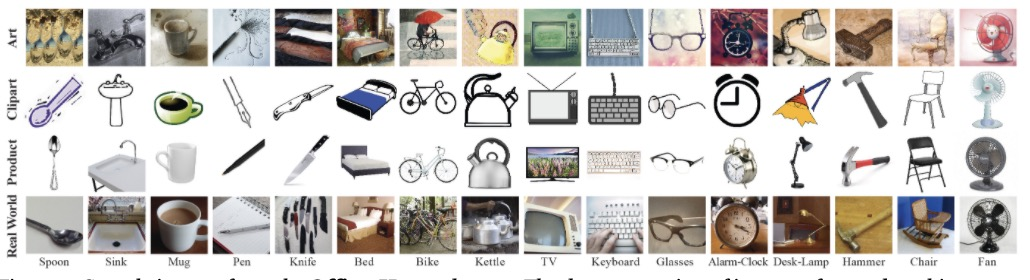
\includegraphics{imgs/dataset.jpg}

    Then, we implement a class to load the data and assign each class a
different label. In addition, we also implement some settings of
one-hot, transformer, balance setting which can be used according to
different model requirements. The following code can show the process:

    \begin{Verbatim}[commandchars=\\\{\}]
{\color{incolor}In [{\color{incolor} }]:} \PY{k}{class} \PY{n+nc}{OfficeHomeDataset}\PY{p}{(}\PY{n}{Dataset}\PY{p}{)}\PY{p}{:}
            \PY{k}{def} \PY{n+nf}{\PYZus{}\PYZus{}init\PYZus{}\PYZus{}}\PY{p}{(}\PY{n+nb+bp}{self}\PY{p}{,} \PY{n}{data\PYZus{}path}\PY{p}{,} \PY{n}{domain}\PY{o}{=}\PY{l+s+s2}{\PYZdq{}}\PY{l+s+s2}{Real World}\PY{l+s+s2}{\PYZdq{}}\PY{p}{,} 
                         \PY{n}{balance}\PY{o}{=}\PY{k+kc}{False}\PY{p}{,} \PY{n}{one\PYZus{}hot}\PY{o}{=}\PY{k+kc}{False}\PY{p}{,} \PY{n}{transform}\PY{o}{=}\PY{k+kc}{None}\PY{p}{)}\PY{p}{:}
                \PY{n+nb+bp}{self}\PY{o}{.}\PY{n}{transform} \PY{o}{=} \PY{n}{transform}
                \PY{n+nb+bp}{self}\PY{o}{.}\PY{n}{domain} \PY{o}{=} \PY{n}{domain}
                \PY{n+nb+bp}{self}\PY{o}{.}\PY{n}{balance} \PY{o}{=} \PY{n}{balance}
                \PY{n+nb+bp}{self}\PY{o}{.}\PY{n}{one\PYZus{}hot} \PY{o}{=} \PY{n}{one\PYZus{}hot}
        
                \PY{c+c1}{\PYZsh{} label dict}
                \PY{n+nb+bp}{self}\PY{o}{.}\PY{n}{label\PYZus{}dict} \PY{o}{=} \PY{p}{\PYZob{}}\PY{l+s+s2}{\PYZdq{}}\PY{l+s+s2}{Art}\PY{l+s+s2}{\PYZdq{}}\PY{p}{:} \PY{l+m+mi}{0}\PY{p}{,} \PY{l+s+s2}{\PYZdq{}}\PY{l+s+s2}{Clipart}\PY{l+s+s2}{\PYZdq{}}\PY{p}{:}\PY{l+m+mi}{1}\PY{p}{,} \PY{l+s+s2}{\PYZdq{}}\PY{l+s+s2}{Product}\PY{l+s+s2}{\PYZdq{}}\PY{p}{:}\PY{l+m+mi}{2}\PY{p}{,} \PY{l+s+s1}{\PYZsq{}}\PY{l+s+s1}{Real World}\PY{l+s+s1}{\PYZsq{}}\PY{p}{:} \PY{l+m+mi}{3}\PY{p}{\PYZcb{}}
        
                \PY{c+c1}{\PYZsh{} Read all file names}
                \PY{n+nb+bp}{self}\PY{o}{.}\PY{n}{file\PYZus{}names} \PY{o}{=} \PY{p}{[}\PY{p}{]}
                \PY{k}{if} \PY{n+nb+bp}{self}\PY{o}{.}\PY{n}{domain} \PY{o+ow}{is} \PY{k+kc}{None}\PY{p}{:}
                    \PY{n+nb+bp}{self}\PY{o}{.}\PY{n}{n\PYZus{}classes} \PY{o}{=} \PY{l+m+mi}{3}
                    \PY{k}{for} \PY{n}{root}\PY{p}{,} \PY{n}{dirs}\PY{p}{,} \PY{n}{files} \PY{o+ow}{in} \PY{n}{os}\PY{o}{.}\PY{n}{walk}\PY{p}{(}\PY{n}{data\PYZus{}path}\PY{p}{)}\PY{p}{:}
                        \PY{k}{for} \PY{n}{filename} \PY{o+ow}{in} \PY{n}{files}\PY{p}{:}
                            \PY{k}{if} \PY{n}{filename} \PY{o}{==} \PY{l+s+s2}{\PYZdq{}}\PY{l+s+s2}{.DS\PYZus{}Store}\PY{l+s+s2}{\PYZdq{}}\PY{p}{:} \PY{k}{continue}
                            \PY{k}{elif} \PY{n}{os}\PY{o}{.}\PY{n}{path}\PY{o}{.}\PY{n}{splitext}\PY{p}{(}\PY{n}{filename}\PY{p}{)}\PY{p}{[}\PY{o}{\PYZhy{}}\PY{l+m+mi}{1}\PY{p}{]} \PY{o}{==} \PY{l+s+s2}{\PYZdq{}}\PY{l+s+s2}{.txt}\PY{l+s+s2}{\PYZdq{}}\PY{p}{:} \PY{k}{continue}
                            \PY{n+nb+bp}{self}\PY{o}{.}\PY{n}{file\PYZus{}names}\PY{o}{.}\PY{n}{append}\PY{p}{(}\PY{n}{os}\PY{o}{.}\PY{n}{path}\PY{o}{.}\PY{n}{join}\PY{p}{(}\PY{n}{root}\PY{p}{,} \PY{n}{filename}\PY{p}{)}\PY{p}{)}
                \PY{k}{else}\PY{p}{:}
                    \PY{n+nb+bp}{self}\PY{o}{.}\PY{n}{n\PYZus{}classes} \PY{o}{=} \PY{l+m+mi}{2}
                    \PY{n}{domain\PYZus{}file} \PY{o}{=} \PY{p}{[}\PY{p}{]}
                    \PY{n}{source\PYZus{}file} \PY{o}{=} \PY{p}{[}\PY{p}{]}
                    \PY{k}{for} \PY{n}{root}\PY{p}{,} \PY{n}{dirs}\PY{p}{,} \PY{n}{files} \PY{o+ow}{in} \PY{n}{os}\PY{o}{.}\PY{n}{walk}\PY{p}{(}\PY{n}{data\PYZus{}path}\PY{p}{)}\PY{p}{:}
                        \PY{k}{if} \PY{n+nb+bp}{self}\PY{o}{.}\PY{n}{domain} \PY{o+ow}{in} \PY{n}{root}\PY{p}{:}
                            \PY{k}{for} \PY{n}{filename} \PY{o+ow}{in} \PY{n}{files}\PY{p}{:}
                                \PY{k}{if} \PY{n}{filename} \PY{o}{==} \PY{l+s+s2}{\PYZdq{}}\PY{l+s+s2}{.DS\PYZus{}Store}\PY{l+s+s2}{\PYZdq{}}\PY{p}{:} \PY{k}{continue}
                                \PY{k}{elif} \PY{n}{os}\PY{o}{.}\PY{n}{path}\PY{o}{.}\PY{n}{splitext}\PY{p}{(}\PY{n}{filename}\PY{p}{)}\PY{p}{[}\PY{o}{\PYZhy{}}\PY{l+m+mi}{1}\PY{p}{]} \PY{o}{==} \PY{l+s+s2}{\PYZdq{}}\PY{l+s+s2}{.txt}\PY{l+s+s2}{\PYZdq{}}\PY{p}{:} \PY{k}{continue}
                                \PY{n}{domain\PYZus{}file}\PY{o}{.}\PY{n}{append}\PY{p}{(}\PY{n}{os}\PY{o}{.}\PY{n}{path}\PY{o}{.}\PY{n}{join}\PY{p}{(}\PY{n}{root}\PY{p}{,} \PY{n}{filename}\PY{p}{)}\PY{p}{)}
                        \PY{k}{else}\PY{p}{:}
                            \PY{k}{for} \PY{n}{filename} \PY{o+ow}{in} \PY{n}{files}\PY{p}{:}
                                \PY{k}{if} \PY{n}{filename} \PY{o}{==} \PY{l+s+s2}{\PYZdq{}}\PY{l+s+s2}{.DS\PYZus{}Store}\PY{l+s+s2}{\PYZdq{}}\PY{p}{:} \PY{k}{continue}
                                \PY{k}{elif} \PY{n}{os}\PY{o}{.}\PY{n}{path}\PY{o}{.}\PY{n}{splitext}\PY{p}{(}\PY{n}{filename}\PY{p}{)}\PY{p}{[}\PY{o}{\PYZhy{}}\PY{l+m+mi}{1}\PY{p}{]} \PY{o}{==} \PY{l+s+s2}{\PYZdq{}}\PY{l+s+s2}{.txt}\PY{l+s+s2}{\PYZdq{}}\PY{p}{:} \PY{k}{continue}
                                \PY{n}{source\PYZus{}file}\PY{o}{.}\PY{n}{append}\PY{p}{(}\PY{n}{os}\PY{o}{.}\PY{n}{path}\PY{o}{.}\PY{n}{join}\PY{p}{(}\PY{n}{root}\PY{p}{,} \PY{n}{filename}\PY{p}{)}\PY{p}{)}
                    \PY{k}{if} \PY{n}{balance}\PY{p}{:}
                        \PY{n+nb+bp}{self}\PY{o}{.}\PY{n}{file\PYZus{}names} \PY{o}{=} \PY{n}{domain\PYZus{}file} \PY{o}{+} \PY{n}{sample}\PY{p}{(}\PY{n}{source\PYZus{}file}\PY{p}{,} \PY{n+nb}{len}\PY{p}{(}\PY{n}{domain\PYZus{}file}\PY{p}{)}\PY{p}{)}
                    \PY{k}{else}\PY{p}{:}
                        \PY{n+nb+bp}{self}\PY{o}{.}\PY{n}{file\PYZus{}names} \PY{o}{=} \PY{n}{domain\PYZus{}file} \PY{o}{+} \PY{n}{source\PYZus{}file}
                
                \PY{n+nb}{print}\PY{p}{(}\PY{n+nb}{len}\PY{p}{(}\PY{n+nb+bp}{self}\PY{o}{.}\PY{n}{file\PYZus{}names}\PY{p}{)}\PY{p}{)}
                \PY{c+c1}{\PYZsh{} self.file\PYZus{}names = sample(self.file\PYZus{}names, 200)}
        
            \PY{k}{def} \PY{n+nf}{\PYZus{}\PYZus{}len\PYZus{}\PYZus{}}\PY{p}{(}\PY{n+nb+bp}{self}\PY{p}{)}\PY{p}{:}
                \PY{k}{return} \PY{n+nb}{len}\PY{p}{(}\PY{n+nb+bp}{self}\PY{o}{.}\PY{n}{file\PYZus{}names}\PY{p}{)}
        
            \PY{k}{def} \PY{n+nf}{\PYZus{}\PYZus{}getitem\PYZus{}\PYZus{}}\PY{p}{(}\PY{n+nb+bp}{self}\PY{p}{,} \PY{n}{idx}\PY{p}{)}\PY{p}{:}
                \PY{k}{if} \PY{n}{torch}\PY{o}{.}\PY{n}{is\PYZus{}tensor}\PY{p}{(}\PY{n}{idx}\PY{p}{)}\PY{p}{:}
                    \PY{n}{idx} \PY{o}{=} \PY{n}{idx}\PY{o}{.}\PY{n}{tolist}\PY{p}{(}\PY{p}{)}
        
                \PY{n}{label} \PY{o}{=} \PY{p}{[}\PY{p}{]}
                \PY{n}{filename} \PY{o}{=} \PY{n+nb+bp}{self}\PY{o}{.}\PY{n}{file\PYZus{}names}\PY{p}{[}\PY{n}{idx}\PY{p}{]}
                \PY{n}{img} \PY{o}{=} \PY{n}{Image}\PY{o}{.}\PY{n}{open}\PY{p}{(}\PY{n}{filename}\PY{p}{)}
                \PY{k}{if} \PY{n+nb+bp}{self}\PY{o}{.}\PY{n}{transform}\PY{p}{:}
                    \PY{n}{img} \PY{o}{=} \PY{n+nb+bp}{self}\PY{o}{.}\PY{n}{transform}\PY{p}{(}\PY{n}{img}\PY{p}{)}
                \PY{c+c1}{\PYZsh{} print(img.shape, filename)}
                \PY{n}{source\PYZus{}name} \PY{o}{=} \PY{n}{filename}\PY{o}{.}\PY{n}{split}\PY{p}{(}\PY{l+s+s1}{\PYZsq{}}\PY{l+s+s1}{/}\PY{l+s+s1}{\PYZsq{}}\PY{p}{)}\PY{p}{[}\PY{o}{\PYZhy{}}\PY{l+m+mi}{3}\PY{p}{]}
                \PY{k}{if} \PY{n+nb+bp}{self}\PY{o}{.}\PY{n}{domain} \PY{o+ow}{is} \PY{k+kc}{None}\PY{p}{:}
                    \PY{n}{label}\PY{o}{.}\PY{n}{append}\PY{p}{(}\PY{n+nb+bp}{self}\PY{o}{.}\PY{n}{label\PYZus{}dict}\PY{p}{[}\PY{n}{source\PYZus{}name}\PY{p}{]}\PY{p}{)}
                \PY{k}{else}\PY{p}{:}
                    \PY{k}{if} \PY{n}{source\PYZus{}name} \PY{o}{==} \PY{n+nb+bp}{self}\PY{o}{.}\PY{n}{domain}\PY{p}{:}
                        \PY{n}{label}\PY{o}{.}\PY{n}{append}\PY{p}{(}\PY{l+m+mi}{1}\PY{p}{)}
                    \PY{k}{else}\PY{p}{:} \PY{n}{label}\PY{o}{.}\PY{n}{append}\PY{p}{(}\PY{l+m+mi}{0}\PY{p}{)}
                \PY{k}{if} \PY{n+nb+bp}{self}\PY{o}{.}\PY{n}{one\PYZus{}hot}\PY{p}{:}
                    \PY{n}{label} \PY{o}{=} \PY{n}{np}\PY{o}{.}\PY{n}{array}\PY{p}{(}\PY{n}{label}\PY{p}{)}
                    \PY{n}{label} \PY{o}{=} \PY{n}{np}\PY{o}{.}\PY{n}{eye}\PY{p}{(}\PY{n+nb+bp}{self}\PY{o}{.}\PY{n}{n\PYZus{}classes}\PY{p}{)}\PY{p}{[}\PY{n}{label}\PY{p}{]}
                    \PY{n}{label} \PY{o}{=} \PY{n}{np}\PY{o}{.}\PY{n}{float32}\PY{p}{(}\PY{n}{label}\PY{p}{)}
                \PY{k}{else}\PY{p}{:}
                    \PY{n}{label} \PY{o}{=} \PY{n}{np}\PY{o}{.}\PY{n}{array}\PY{p}{(}\PY{n}{label}\PY{p}{)}
                \PY{c+c1}{\PYZsh{} sample = \PYZob{}\PYZsq{}image\PYZsq{}: img, \PYZsq{}label\PYZsq{}: label\PYZcb{}}
                \PY{n}{sample} \PY{o}{=} \PY{p}{[}\PY{n}{img}\PY{p}{,} \PY{n}{label}\PY{p}{]}
        
                \PY{k}{return} \PY{n}{sample}
\end{Verbatim}


    And we used two ways to create dataloaders, they are used for class
classification and domain classification tasks separately:

    \begin{Verbatim}[commandchars=\\\{\}]
{\color{incolor}In [{\color{incolor} }]:} \PY{c+c1}{\PYZsh{} These two methods are used for class classification}
        \PY{k}{def} \PY{n+nf}{load\PYZus{}training}\PY{p}{(}\PY{n}{root\PYZus{}path}\PY{p}{,} \PY{n+nb}{dir}\PY{p}{,} \PY{n}{batch\PYZus{}size}\PY{p}{,} \PY{n}{kwargs}\PY{p}{)}\PY{p}{:}
            \PY{n}{transform} \PY{o}{=} \PY{n}{transforms}\PY{o}{.}\PY{n}{Compose}\PY{p}{(}
                \PY{p}{[}\PY{n}{transforms}\PY{o}{.}\PY{n}{Resize}\PY{p}{(}\PY{p}{[}\PY{l+m+mi}{256}\PY{p}{,} \PY{l+m+mi}{256}\PY{p}{]}\PY{p}{)}\PY{p}{,}
                 \PY{n}{transforms}\PY{o}{.}\PY{n}{RandomCrop}\PY{p}{(}\PY{l+m+mi}{224}\PY{p}{)}\PY{p}{,}
                 \PY{n}{transforms}\PY{o}{.}\PY{n}{RandomHorizontalFlip}\PY{p}{(}\PY{p}{)}\PY{p}{,}
                 \PY{n}{transforms}\PY{o}{.}\PY{n}{ToTensor}\PY{p}{(}\PY{p}{)}\PY{p}{]}\PY{p}{)}
            \PY{n}{data} \PY{o}{=} \PY{n}{datasets}\PY{o}{.}\PY{n}{ImageFolder}\PY{p}{(}\PY{n}{root}\PY{o}{=}\PY{n}{os}\PY{o}{.}\PY{n}{path}\PY{o}{.}\PY{n}{join}\PY{p}{(}\PY{n}{root\PYZus{}path}\PY{p}{,} \PY{n+nb}{dir}\PY{p}{)}\PY{p}{,} 
                                        \PY{n}{transform}\PY{o}{=}\PY{n}{transform}\PY{p}{)}
            \PY{n}{train\PYZus{}loader} \PY{o}{=} \PY{n}{torch}\PY{o}{.}\PY{n}{utils}\PY{o}{.}\PY{n}{data}\PY{o}{.}\PY{n}{DataLoader}\PY{p}{(}
                \PY{n}{data}\PY{p}{,} \PY{n}{batch\PYZus{}size}\PY{o}{=}\PY{n}{batch\PYZus{}size}\PY{p}{,} 
                \PY{n}{shuffle}\PY{o}{=}\PY{k+kc}{True}\PY{p}{,} \PY{n}{drop\PYZus{}last}\PY{o}{=}\PY{k+kc}{True}\PY{p}{,} \PY{o}{*}\PY{o}{*}\PY{n}{kwargs}\PY{p}{)}
            \PY{k}{return} \PY{n}{train\PYZus{}loader}
        
        \PY{k}{def} \PY{n+nf}{load\PYZus{}testing}\PY{p}{(}\PY{n}{root\PYZus{}path}\PY{p}{,} \PY{n+nb}{dir}\PY{p}{,} \PY{n}{batch\PYZus{}size}\PY{p}{,} \PY{n}{kwargs}\PY{p}{)}\PY{p}{:}
            \PY{n}{transform} \PY{o}{=} \PY{n}{transforms}\PY{o}{.}\PY{n}{Compose}\PY{p}{(}
                \PY{p}{[}\PY{n}{transforms}\PY{o}{.}\PY{n}{Resize}\PY{p}{(}\PY{p}{[}\PY{l+m+mi}{224}\PY{p}{,} \PY{l+m+mi}{224}\PY{p}{]}\PY{p}{)}\PY{p}{,}
                 \PY{n}{transforms}\PY{o}{.}\PY{n}{ToTensor}\PY{p}{(}\PY{p}{)}\PY{p}{]}\PY{p}{)}
            \PY{n}{data} \PY{o}{=} \PY{n}{datasets}\PY{o}{.}\PY{n}{ImageFolder}\PY{p}{(}\PY{n}{root}\PY{o}{=}\PY{n}{os}\PY{o}{.}\PY{n}{path}\PY{o}{.}\PY{n}{join}\PY{p}{(}\PY{n}{root\PYZus{}path}\PY{p}{,} \PY{n+nb}{dir}\PY{p}{)}\PY{p}{,} 
                                        \PY{n}{transform}\PY{o}{=}\PY{n}{transform}\PY{p}{)}
            \PY{n}{test\PYZus{}loader} \PY{o}{=} \PY{n}{torch}\PY{o}{.}\PY{n}{utils}\PY{o}{.}\PY{n}{data}\PY{o}{.}\PY{n}{DataLoader}\PY{p}{(}
                \PY{n}{data}\PY{p}{,} \PY{n}{batch\PYZus{}size}\PY{o}{=}\PY{n}{batch\PYZus{}size}\PY{p}{,} 
                \PY{n}{shuffle}\PY{o}{=}\PY{k+kc}{True}\PY{p}{,} \PY{o}{*}\PY{o}{*}\PY{n}{kwargs}\PY{p}{)}
            \PY{k}{return} \PY{n}{test\PYZus{}loader}
\end{Verbatim}


    \begin{Verbatim}[commandchars=\\\{\}]
{\color{incolor}In [{\color{incolor}1}]:} \PY{c+c1}{\PYZsh{} These two methods are used for domain classification}
        \PY{k}{def} \PY{n+nf}{load\PYZus{}training}\PY{p}{(}\PY{n}{root\PYZus{}path}\PY{p}{,} \PY{n+nb}{dir}\PY{p}{,} \PY{n}{batch\PYZus{}size}\PY{p}{,} \PY{n}{kwargs}\PY{p}{)}\PY{p}{:}
            \PY{n}{transform} \PY{o}{=} \PY{n}{transforms}\PY{o}{.}\PY{n}{Compose}\PY{p}{(}
                \PY{p}{[}\PY{n}{transforms}\PY{o}{.}\PY{n}{Resize}\PY{p}{(}\PY{p}{[}\PY{l+m+mi}{256}\PY{p}{,} \PY{l+m+mi}{256}\PY{p}{]}\PY{p}{)}\PY{p}{,}
                 \PY{n}{transforms}\PY{o}{.}\PY{n}{RandomCrop}\PY{p}{(}\PY{l+m+mi}{224}\PY{p}{)}\PY{p}{,}
                 \PY{n}{transforms}\PY{o}{.}\PY{n}{RandomHorizontalFlip}\PY{p}{(}\PY{p}{)}\PY{p}{,}
                 \PY{n}{transforms}\PY{o}{.}\PY{n}{ToTensor}\PY{p}{(}\PY{p}{)}\PY{p}{]}\PY{p}{)}
            \PY{n}{data} \PY{o}{=} \PY{n}{OfficeHomeDataset}\PY{p}{(}\PY{n}{os}\PY{o}{.}\PY{n}{path}\PY{o}{.}\PY{n}{join}\PY{p}{(}\PY{n}{root\PYZus{}path}\PY{p}{,} \PY{n+nb}{dir}\PY{p}{)}\PY{p}{,} 
                                     \PY{n}{transform}\PY{o}{=}\PY{n}{transform}\PY{p}{)}
            \PY{n}{train\PYZus{}loader} \PY{o}{=} \PY{n}{torch}\PY{o}{.}\PY{n}{utils}\PY{o}{.}\PY{n}{data}\PY{o}{.}\PY{n}{DataLoader}\PY{p}{(}
                \PY{n}{data}\PY{p}{,} \PY{n}{batch\PYZus{}size}\PY{o}{=}\PY{n}{batch\PYZus{}size}\PY{p}{,} 
                \PY{n}{shuffle}\PY{o}{=}\PY{k+kc}{True}\PY{p}{,} \PY{n}{drop\PYZus{}last}\PY{o}{=}\PY{k+kc}{True}\PY{p}{,} \PY{o}{*}\PY{o}{*}\PY{n}{kwargs}\PY{p}{)}
            \PY{k}{return} \PY{n}{train\PYZus{}loader}
        
        \PY{k}{def} \PY{n+nf}{load\PYZus{}testing}\PY{p}{(}\PY{n}{root\PYZus{}path}\PY{p}{,} \PY{n+nb}{dir}\PY{p}{,} \PY{n}{batch\PYZus{}size}\PY{p}{,} \PY{n}{kwargs}\PY{p}{)}\PY{p}{:}
            \PY{n}{transform} \PY{o}{=} \PY{n}{transforms}\PY{o}{.}\PY{n}{Compose}\PY{p}{(}
                \PY{p}{[}\PY{n}{transforms}\PY{o}{.}\PY{n}{Resize}\PY{p}{(}\PY{p}{[}\PY{l+m+mi}{224}\PY{p}{,} \PY{l+m+mi}{224}\PY{p}{]}\PY{p}{)}\PY{p}{,}
                 \PY{n}{transforms}\PY{o}{.}\PY{n}{ToTensor}\PY{p}{(}\PY{p}{)}\PY{p}{]}\PY{p}{)}
            \PY{n}{data} \PY{o}{=} \PY{n}{OfficeHomeDataset}\PY{p}{(}\PY{n}{os}\PY{o}{.}\PY{n}{path}\PY{o}{.}\PY{n}{join}\PY{p}{(}\PY{n}{root\PYZus{}path}\PY{p}{,} \PY{n+nb}{dir}\PY{p}{)}\PY{p}{,} 
                                     \PY{n}{transform}\PY{o}{=}\PY{n}{transform}\PY{p}{)}
            \PY{n}{test\PYZus{}loader} \PY{o}{=} \PY{n}{torch}\PY{o}{.}\PY{n}{utils}\PY{o}{.}\PY{n}{data}\PY{o}{.}\PY{n}{DataLoader}\PY{p}{(}
                \PY{n}{data}\PY{p}{,} \PY{n}{batch\PYZus{}size}\PY{o}{=}\PY{n}{batch\PYZus{}size}\PY{p}{,} 
                \PY{n}{shuffle}\PY{o}{=}\PY{k+kc}{True}\PY{p}{,} \PY{o}{*}\PY{o}{*}\PY{n}{kwargs}\PY{p}{)}
            \PY{k}{return} \PY{n}{test\PYZus{}loader}
\end{Verbatim}


    \hypertarget{model-stucture}{%
\subsection{Model stucture}\label{model-stucture}}

In the pre-adaptation stage, we need to train a source-specific feature
extractor \(F_{si}\) and a source-specificclassifier \(Q_{si}\) for each
specific source \(S_i\). For the domain, there is a
domainclassifier(\(D_{Si}\)) to be trained. In addition, in the second
stage, the weighted aligned source encoder \(E_{Si}\) for each source
\(S_i\), and the target encoder \(E_T\) as well as the target classifier
\(Q_T\) need to be trained. The following section is going to describe
each model struture in details.

    \hypertarget{feature-extractor-and-source-specificclassifier}{%
\subsubsection{Feature Extractor and
Source-specificclassifier}\label{feature-extractor-and-source-specificclassifier}}

The archtercture of the \(F_{si}\) is implemented by the following
layers:

\begin{itemize}
\tightlist
\item
  ImageNet pre-trained ResNet-50 till average pool layer
\item
  Linear FC (2048, 1024) + ELU
\item
  Linear FC (1024, 1024) + BatchNorm + ELU
\item
  Linear FC (1024, f \_dim) + ELU
\item
  Linear FC ( f \_dim, f \_dim) + BatchNorm + ELU
\end{itemize}

For the source-specificclassifier \(Q_{si}\), It adds a layer on the
basis of feature extractor

\begin{itemize}
\tightlist
\item
  LinearFC(f\_dim,3)
\end{itemize}

We used pretrained Resnet model for the first layer, and the training
details for Office-Home can be found in the appendix of the original
paper. Our implementaion of the Feature extrator and the
source-specificclassifier can be found as follings:

    \begin{Verbatim}[commandchars=\\\{\}]
{\color{incolor}In [{\color{incolor} }]:}   \PY{k}{class} \PY{n+nc}{SourceClassifer}\PY{p}{(}\PY{n}{nn}\PY{o}{.}\PY{n}{Module}\PY{p}{)}\PY{p}{:}
            \PY{k}{def} \PY{n+nf}{\PYZus{}\PYZus{}init\PYZus{}\PYZus{}}\PY{p}{(}\PY{n+nb+bp}{self}\PY{p}{,} \PY{n}{f\PYZus{}dim}\PY{o}{=}\PY{l+m+mi}{256}\PY{p}{,} \PY{n}{n\PYZus{}classes}\PY{o}{=}\PY{l+m+mi}{65}\PY{p}{)}\PY{p}{:}
                \PY{n+nb}{super}\PY{p}{(}\PY{n}{SourceClassifer}\PY{p}{,} \PY{n+nb+bp}{self}\PY{p}{)}\PY{o}{.}\PY{n+nf+fm}{\PYZus{}\PYZus{}init\PYZus{}\PYZus{}}\PY{p}{(}\PY{p}{)}
        
                \PY{n+nb+bp}{self}\PY{o}{.}\PY{n}{f\PYZus{}dim} \PY{o}{=} \PY{n}{f\PYZus{}dim}
                \PY{n+nb+bp}{self}\PY{o}{.}\PY{n}{n\PYZus{}classes} \PY{o}{=} \PY{n}{n\PYZus{}classes}
        
                \PY{c+c1}{\PYZsh{} Get ResNet50 model}
                \PY{n}{ResNet50} \PY{o}{=} \PY{n}{torch}\PY{o}{.}\PY{n}{hub}\PY{o}{.}\PY{n}{load}\PY{p}{(}\PY{l+s+s1}{\PYZsq{}}\PY{l+s+s1}{pytorch/vision:v0.6.0}\PY{l+s+s1}{\PYZsq{}}\PY{p}{,} 
                                          \PY{l+s+s1}{\PYZsq{}}\PY{l+s+s1}{resnet50}\PY{l+s+s1}{\PYZsq{}}\PY{p}{,} \PY{n}{pretrained}\PY{o}{=}\PY{k+kc}{False}\PY{p}{)}
                \PY{n}{ResNet50}\PY{o}{.}\PY{n}{fc} \PY{o}{=} \PY{n}{nn}\PY{o}{.}\PY{n}{Identity}\PY{p}{(}\PY{p}{)}
                \PY{n+nb+bp}{self}\PY{o}{.}\PY{n}{ResNet50} \PY{o}{=} \PY{n}{ResNet50}
        
                \PY{n+nb+bp}{self}\PY{o}{.}\PY{n}{extractor1} \PY{o}{=} \PY{n}{nn}\PY{o}{.}\PY{n}{Sequential}\PY{p}{(}
                    \PY{n}{nn}\PY{o}{.}\PY{n}{Linear}\PY{p}{(}\PY{l+m+mi}{2048}\PY{p}{,} \PY{l+m+mi}{1024}\PY{p}{)}\PY{p}{,}
                    \PY{n}{nn}\PY{o}{.}\PY{n}{ELU}\PY{p}{(}\PY{p}{)}\PY{p}{,}
                    \PY{n}{nn}\PY{o}{.}\PY{n}{Linear}\PY{p}{(}\PY{l+m+mi}{1024}\PY{p}{,} \PY{l+m+mi}{1024}\PY{p}{)}\PY{p}{,}
                    \PY{n}{nn}\PY{o}{.}\PY{n}{BatchNorm1d}\PY{p}{(}\PY{l+m+mi}{1024}\PY{p}{)}\PY{p}{,}  \PY{c+c1}{\PYZsh{} expect 2\PYZhy{}D input}
                    \PY{n}{nn}\PY{o}{.}\PY{n}{ELU}\PY{p}{(}\PY{p}{)}\PY{p}{,}
                    \PY{n}{nn}\PY{o}{.}\PY{n}{Linear}\PY{p}{(}\PY{l+m+mi}{1024}\PY{p}{,} \PY{n+nb+bp}{self}\PY{o}{.}\PY{n}{f\PYZus{}dim}\PY{p}{)}\PY{p}{,}
                    \PY{n}{nn}\PY{o}{.}\PY{n}{ELU}\PY{p}{(}\PY{p}{)}\PY{p}{,}
                    \PY{n}{nn}\PY{o}{.}\PY{n}{Linear}\PY{p}{(}\PY{n+nb+bp}{self}\PY{o}{.}\PY{n}{f\PYZus{}dim}\PY{p}{,} \PY{n+nb+bp}{self}\PY{o}{.}\PY{n}{f\PYZus{}dim}\PY{p}{)}\PY{p}{,}
                    \PY{n}{nn}\PY{o}{.}\PY{n}{BatchNorm1d}\PY{p}{(}\PY{n+nb+bp}{self}\PY{o}{.}\PY{n}{f\PYZus{}dim}\PY{p}{)}\PY{p}{,}
                    \PY{n}{nn}\PY{o}{.}\PY{n}{ELU}\PY{p}{(}\PY{p}{)}
                \PY{p}{)}
        
                \PY{n+nb+bp}{self}\PY{o}{.}\PY{n}{extractor2} \PY{o}{=} \PY{n}{nn}\PY{o}{.}\PY{n}{Sequential}\PY{p}{(}
                    \PY{n}{nn}\PY{o}{.}\PY{n}{Linear}\PY{p}{(}\PY{l+m+mi}{2048}\PY{p}{,} \PY{l+m+mi}{1024}\PY{p}{)}\PY{p}{,}
                    \PY{n}{nn}\PY{o}{.}\PY{n}{ELU}\PY{p}{(}\PY{p}{)}\PY{p}{,}
                    \PY{n}{nn}\PY{o}{.}\PY{n}{Linear}\PY{p}{(}\PY{l+m+mi}{1024}\PY{p}{,} \PY{l+m+mi}{1024}\PY{p}{)}\PY{p}{,}
                    \PY{n}{nn}\PY{o}{.}\PY{n}{BatchNorm1d}\PY{p}{(}\PY{l+m+mi}{1024}\PY{p}{)}\PY{p}{,}  \PY{c+c1}{\PYZsh{} expect 2\PYZhy{}D input}
                    \PY{n}{nn}\PY{o}{.}\PY{n}{ELU}\PY{p}{(}\PY{p}{)}\PY{p}{,}
                    \PY{n}{nn}\PY{o}{.}\PY{n}{Linear}\PY{p}{(}\PY{l+m+mi}{1024}\PY{p}{,} \PY{n+nb+bp}{self}\PY{o}{.}\PY{n}{f\PYZus{}dim}\PY{p}{)}\PY{p}{,}
                    \PY{n}{nn}\PY{o}{.}\PY{n}{ELU}\PY{p}{(}\PY{p}{)}\PY{p}{,}
                    \PY{n}{nn}\PY{o}{.}\PY{n}{Linear}\PY{p}{(}\PY{n+nb+bp}{self}\PY{o}{.}\PY{n}{f\PYZus{}dim}\PY{p}{,} \PY{n+nb+bp}{self}\PY{o}{.}\PY{n}{f\PYZus{}dim}\PY{p}{)}\PY{p}{,}
                    \PY{n}{nn}\PY{o}{.}\PY{n}{BatchNorm1d}\PY{p}{(}\PY{n+nb+bp}{self}\PY{o}{.}\PY{n}{f\PYZus{}dim}\PY{p}{)}\PY{p}{,}
                    \PY{n}{nn}\PY{o}{.}\PY{n}{ELU}\PY{p}{(}\PY{p}{)}
                \PY{p}{)}
        
                \PY{n+nb+bp}{self}\PY{o}{.}\PY{n}{extractor3} \PY{o}{=} \PY{n}{nn}\PY{o}{.}\PY{n}{Sequential}\PY{p}{(}
                    \PY{n}{nn}\PY{o}{.}\PY{n}{Linear}\PY{p}{(}\PY{l+m+mi}{2048}\PY{p}{,} \PY{l+m+mi}{1024}\PY{p}{)}\PY{p}{,}
                    \PY{n}{nn}\PY{o}{.}\PY{n}{ELU}\PY{p}{(}\PY{p}{)}\PY{p}{,}
                    \PY{n}{nn}\PY{o}{.}\PY{n}{Linear}\PY{p}{(}\PY{l+m+mi}{1024}\PY{p}{,} \PY{l+m+mi}{1024}\PY{p}{)}\PY{p}{,}
                    \PY{n}{nn}\PY{o}{.}\PY{n}{BatchNorm1d}\PY{p}{(}\PY{l+m+mi}{1024}\PY{p}{)}\PY{p}{,}  \PY{c+c1}{\PYZsh{} expect 2\PYZhy{}D input}
                    \PY{n}{nn}\PY{o}{.}\PY{n}{ELU}\PY{p}{(}\PY{p}{)}\PY{p}{,}
                    \PY{n}{nn}\PY{o}{.}\PY{n}{Linear}\PY{p}{(}\PY{l+m+mi}{1024}\PY{p}{,} \PY{n+nb+bp}{self}\PY{o}{.}\PY{n}{f\PYZus{}dim}\PY{p}{)}\PY{p}{,}
                    \PY{n}{nn}\PY{o}{.}\PY{n}{ELU}\PY{p}{(}\PY{p}{)}\PY{p}{,}
                    \PY{n}{nn}\PY{o}{.}\PY{n}{Linear}\PY{p}{(}\PY{n+nb+bp}{self}\PY{o}{.}\PY{n}{f\PYZus{}dim}\PY{p}{,} \PY{n+nb+bp}{self}\PY{o}{.}\PY{n}{f\PYZus{}dim}\PY{p}{)}\PY{p}{,}
                    \PY{n}{nn}\PY{o}{.}\PY{n}{BatchNorm1d}\PY{p}{(}\PY{n+nb+bp}{self}\PY{o}{.}\PY{n}{f\PYZus{}dim}\PY{p}{)}\PY{p}{,}
                    \PY{n}{nn}\PY{o}{.}\PY{n}{ELU}\PY{p}{(}\PY{p}{)}
                \PY{p}{)}
        
                \PY{n+nb+bp}{self}\PY{o}{.}\PY{n}{cls1} \PY{o}{=} \PY{n}{nn}\PY{o}{.}\PY{n}{Linear}\PY{p}{(}\PY{n+nb+bp}{self}\PY{o}{.}\PY{n}{f\PYZus{}dim}\PY{p}{,} \PY{n+nb+bp}{self}\PY{o}{.}\PY{n}{n\PYZus{}classes}\PY{p}{)}
                \PY{n+nb+bp}{self}\PY{o}{.}\PY{n}{cls2} \PY{o}{=} \PY{n}{nn}\PY{o}{.}\PY{n}{Linear}\PY{p}{(}\PY{n+nb+bp}{self}\PY{o}{.}\PY{n}{f\PYZus{}dim}\PY{p}{,} \PY{n+nb+bp}{self}\PY{o}{.}\PY{n}{n\PYZus{}classes}\PY{p}{)}
                \PY{n+nb+bp}{self}\PY{o}{.}\PY{n}{cls3} \PY{o}{=} \PY{n}{nn}\PY{o}{.}\PY{n}{Linear}\PY{p}{(}\PY{n+nb+bp}{self}\PY{o}{.}\PY{n}{f\PYZus{}dim}\PY{p}{,} \PY{n+nb+bp}{self}\PY{o}{.}\PY{n}{n\PYZus{}classes}\PY{p}{)}
        
            \PY{k}{def} \PY{n+nf}{forward}\PY{p}{(}\PY{n+nb+bp}{self}\PY{p}{,} \PY{n}{data\PYZus{}src}\PY{p}{,} \PY{n}{label\PYZus{}src} \PY{o}{=} \PY{l+m+mi}{0}\PY{p}{,} \PY{n}{mark} \PY{o}{=} \PY{l+m+mi}{1}\PY{p}{,} \PY{n}{training}\PY{o}{=}\PY{k+kc}{True}\PY{p}{)}\PY{p}{:}
                
                \PY{k}{if} \PY{n}{training} \PY{o}{==} \PY{k+kc}{True}\PY{p}{:}
                    \PY{n}{h1} \PY{o}{=} \PY{n+nb+bp}{self}\PY{o}{.}\PY{n}{ResNet50}\PY{p}{(}\PY{n}{data\PYZus{}src}\PY{p}{)}
                    \PY{n}{h1} \PY{o}{=} \PY{n}{torch}\PY{o}{.}\PY{n}{flatten}\PY{p}{(}\PY{n}{h1}\PY{p}{,} \PY{n}{start\PYZus{}dim}\PY{o}{=}\PY{l+m+mi}{1}\PY{p}{)}  \PY{c+c1}{\PYZsh{} size: (batch\PYZus{}size, dim)}
        
                    \PY{k}{if} \PY{n}{mark} \PY{o}{==} \PY{l+m+mi}{1}\PY{p}{:}
                        \PY{n}{feature1} \PY{o}{=} \PY{n+nb+bp}{self}\PY{o}{.}\PY{n}{extractor1}\PY{p}{(}\PY{n}{h1}\PY{p}{)}
                        \PY{n}{pred1} \PY{o}{=} \PY{n+nb+bp}{self}\PY{o}{.}\PY{n}{cls1}\PY{p}{(}\PY{n}{feature1}\PY{p}{)}
        
                        \PY{n}{cls\PYZus{}loss} \PY{o}{=} \PY{n}{F}\PY{o}{.}\PY{n}{cross\PYZus{}entropy}\PY{p}{(}\PY{n}{pred1}\PY{p}{,} \PY{n}{label\PYZus{}src}\PY{p}{)}
        
                        \PY{k}{return} \PY{n}{cls\PYZus{}loss}
        
                    \PY{k}{if} \PY{n}{mark} \PY{o}{==} \PY{l+m+mi}{2}\PY{p}{:}
                        \PY{n}{feature2} \PY{o}{=} \PY{n+nb+bp}{self}\PY{o}{.}\PY{n}{extractor2}\PY{p}{(}\PY{n}{h1}\PY{p}{)}
                        \PY{n}{pred2} \PY{o}{=} \PY{n+nb+bp}{self}\PY{o}{.}\PY{n}{cls2}\PY{p}{(}\PY{n}{feature2}\PY{p}{)}
        
                        \PY{n}{cls\PYZus{}loss} \PY{o}{=} \PY{n}{F}\PY{o}{.}\PY{n}{cross\PYZus{}entropy}\PY{p}{(}\PY{n}{pred2}\PY{p}{,} \PY{n}{label\PYZus{}src}\PY{p}{)}
        
                        \PY{k}{return} \PY{n}{cls\PYZus{}loss}
        
                    \PY{k}{if} \PY{n}{mark} \PY{o}{==} \PY{l+m+mi}{3}\PY{p}{:}
                        \PY{n}{feature3} \PY{o}{=} \PY{n+nb+bp}{self}\PY{o}{.}\PY{n}{extractor3}\PY{p}{(}\PY{n}{h1}\PY{p}{)}
                        \PY{n}{pred3} \PY{o}{=} \PY{n+nb+bp}{self}\PY{o}{.}\PY{n}{cls3}\PY{p}{(}\PY{n}{feature3}\PY{p}{)}
        
                        \PY{n}{cls\PYZus{}loss} \PY{o}{=} \PY{n}{F}\PY{o}{.}\PY{n}{cross\PYZus{}entropy}\PY{p}{(}\PY{n}{pred3}\PY{p}{,} \PY{n}{label\PYZus{}src}\PY{p}{)}
        
                        \PY{k}{return} \PY{n}{cls\PYZus{}loss}
        
                \PY{k}{else}\PY{p}{:}
                    \PY{n}{h1} \PY{o}{=} \PY{n+nb+bp}{self}\PY{o}{.}\PY{n}{ResNet50}\PY{p}{(}\PY{n}{data\PYZus{}src}\PY{p}{)}
                    \PY{n}{h1} \PY{o}{=} \PY{n}{torch}\PY{o}{.}\PY{n}{flatten}\PY{p}{(}\PY{n}{h1}\PY{p}{,} \PY{n}{start\PYZus{}dim}\PY{o}{=}\PY{l+m+mi}{1}\PY{p}{)}  \PY{c+c1}{\PYZsh{} size: (batch\PYZus{}size, dim)}
        
                    \PY{n}{feature1} \PY{o}{=} \PY{n+nb+bp}{self}\PY{o}{.}\PY{n}{extractor1}\PY{p}{(}\PY{n}{h1}\PY{p}{)}
                    \PY{n}{pred1} \PY{o}{=} \PY{n+nb+bp}{self}\PY{o}{.}\PY{n}{cls1}\PY{p}{(}\PY{n}{feature1}\PY{p}{)}
        
                    \PY{n}{feature2} \PY{o}{=} \PY{n+nb+bp}{self}\PY{o}{.}\PY{n}{extractor2}\PY{p}{(}\PY{n}{h1}\PY{p}{)}
                    \PY{n}{pred2} \PY{o}{=} \PY{n+nb+bp}{self}\PY{o}{.}\PY{n}{cls2}\PY{p}{(}\PY{n}{feature2}\PY{p}{)}
        
                    \PY{n}{feature3} \PY{o}{=} \PY{n+nb+bp}{self}\PY{o}{.}\PY{n}{extractor3}\PY{p}{(}\PY{n}{h1}\PY{p}{)}
                    \PY{n}{pred3} \PY{o}{=} \PY{n+nb+bp}{self}\PY{o}{.}\PY{n}{cls3}\PY{p}{(}\PY{n}{feature3}\PY{p}{)}
        
                    \PY{k}{return} \PY{n}{pred1}\PY{p}{,} \PY{n}{pred2}\PY{p}{,} \PY{n}{pred3}\PY{p}{,} \PY{n}{feature1}\PY{p}{,} \PY{n}{feature2}\PY{p}{,} \PY{n}{feature3}
\end{Verbatim}


    \hypertarget{domain-classifier}{%
\subsubsection{Domain classifier}\label{domain-classifier}}

The architecture of domain classifier adds a extra layer on the
architecture of the feature extractor:

\begin{itemize}
\tightlist
\item
  Linear FC (f\_dim, f\_dim/2) + ELU + Linear FC (f\_dim/2, 2)
\end{itemize}

    \begin{Verbatim}[commandchars=\\\{\}]
{\color{incolor}In [{\color{incolor} }]:} \PY{k}{class} \PY{n+nc}{DomainClassifier}\PY{p}{(}\PY{n}{nn}\PY{o}{.}\PY{n}{Module}\PY{p}{)}\PY{p}{:}
            \PY{k}{def} \PY{n+nf}{\PYZus{}\PYZus{}init\PYZus{}\PYZus{}}\PY{p}{(}\PY{n+nb+bp}{self}\PY{p}{,} \PY{n}{sourceClassifier}\PY{p}{,} \PY{n}{f\PYZus{}dim}\PY{o}{=}\PY{l+m+mi}{256}\PY{p}{,} \PY{n}{n\PYZus{}classes}\PY{o}{=}\PY{l+m+mi}{2}\PY{p}{)}\PY{p}{:}
                \PY{n+nb}{super}\PY{p}{(}\PY{n}{DomainClassifier}\PY{p}{,} \PY{n+nb+bp}{self}\PY{p}{)}\PY{o}{.}\PY{n+nf+fm}{\PYZus{}\PYZus{}init\PYZus{}\PYZus{}}\PY{p}{(}\PY{p}{)}
                \PY{n+nb+bp}{self}\PY{o}{.}\PY{n}{f\PYZus{}dim} \PY{o}{=} \PY{n}{f\PYZus{}dim}
                \PY{n+nb+bp}{self}\PY{o}{.}\PY{n}{half\PYZus{}f\PYZus{}dim} \PY{o}{=} \PY{n+nb+bp}{self}\PY{o}{.}\PY{n}{f\PYZus{}dim} \PY{o}{/}\PY{o}{/} \PY{l+m+mi}{2}
                \PY{n+nb+bp}{self}\PY{o}{.}\PY{n}{n\PYZus{}classes} \PY{o}{=} \PY{n}{n\PYZus{}classes}
        
                \PY{n+nb+bp}{self}\PY{o}{.}\PY{n}{sourceClassifier} \PY{o}{=} \PY{n}{sourceClassifier}
        
                \PY{n+nb+bp}{self}\PY{o}{.}\PY{n}{domain\PYZus{}cls1} \PY{o}{=} \PY{n}{nn}\PY{o}{.}\PY{n}{Sequential}\PY{p}{(}
                    \PY{n}{nn}\PY{o}{.}\PY{n}{Linear}\PY{p}{(}\PY{n+nb+bp}{self}\PY{o}{.}\PY{n}{f\PYZus{}dim}\PY{p}{,} \PY{n+nb+bp}{self}\PY{o}{.}\PY{n}{half\PYZus{}f\PYZus{}dim}\PY{p}{)}\PY{p}{,}
                    \PY{n}{nn}\PY{o}{.}\PY{n}{ELU}\PY{p}{(}\PY{p}{)}\PY{p}{,}
                    \PY{n}{nn}\PY{o}{.}\PY{n}{Linear}\PY{p}{(}\PY{n+nb+bp}{self}\PY{o}{.}\PY{n}{half\PYZus{}f\PYZus{}dim}\PY{p}{,} \PY{n+nb+bp}{self}\PY{o}{.}\PY{n}{n\PYZus{}classes}\PY{p}{)}
                \PY{p}{)}
        
                \PY{n+nb+bp}{self}\PY{o}{.}\PY{n}{domain\PYZus{}cls2} \PY{o}{=} \PY{n}{nn}\PY{o}{.}\PY{n}{Sequential}\PY{p}{(}
                    \PY{n}{nn}\PY{o}{.}\PY{n}{Linear}\PY{p}{(}\PY{n+nb+bp}{self}\PY{o}{.}\PY{n}{f\PYZus{}dim}\PY{p}{,} \PY{n+nb+bp}{self}\PY{o}{.}\PY{n}{half\PYZus{}f\PYZus{}dim}\PY{p}{)}\PY{p}{,}
                    \PY{n}{nn}\PY{o}{.}\PY{n}{ELU}\PY{p}{(}\PY{p}{)}\PY{p}{,}
                    \PY{n}{nn}\PY{o}{.}\PY{n}{Linear}\PY{p}{(}\PY{n+nb+bp}{self}\PY{o}{.}\PY{n}{half\PYZus{}f\PYZus{}dim}\PY{p}{,} \PY{n+nb+bp}{self}\PY{o}{.}\PY{n}{n\PYZus{}classes}\PY{p}{)}
                \PY{p}{)}
        
                \PY{n+nb+bp}{self}\PY{o}{.}\PY{n}{domain\PYZus{}cls3} \PY{o}{=} \PY{n}{nn}\PY{o}{.}\PY{n}{Sequential}\PY{p}{(}
                    \PY{n}{nn}\PY{o}{.}\PY{n}{Linear}\PY{p}{(}\PY{n+nb+bp}{self}\PY{o}{.}\PY{n}{f\PYZus{}dim}\PY{p}{,} \PY{n+nb+bp}{self}\PY{o}{.}\PY{n}{half\PYZus{}f\PYZus{}dim}\PY{p}{)}\PY{p}{,}
                    \PY{n}{nn}\PY{o}{.}\PY{n}{ELU}\PY{p}{(}\PY{p}{)}\PY{p}{,}
                    \PY{n}{nn}\PY{o}{.}\PY{n}{Linear}\PY{p}{(}\PY{n+nb+bp}{self}\PY{o}{.}\PY{n}{half\PYZus{}f\PYZus{}dim}\PY{p}{,} \PY{n+nb+bp}{self}\PY{o}{.}\PY{n}{n\PYZus{}classes}\PY{p}{)}
                \PY{p}{)}
                
            \PY{k}{def} \PY{n+nf}{forward}\PY{p}{(}\PY{n+nb+bp}{self}\PY{p}{,} \PY{n}{data\PYZus{}src}\PY{p}{,} \PY{n}{data\PYZus{}tgt}\PY{o}{=}\PY{k+kc}{None}\PY{p}{,} 
                        \PY{n}{label\PYZus{}src}\PY{o}{=}\PY{l+m+mi}{0}\PY{p}{,} \PY{n}{label\PYZus{}tgt}\PY{o}{=}\PY{l+m+mi}{0}\PY{p}{,} \PY{n}{mark}\PY{o}{=}\PY{l+m+mi}{1}\PY{p}{,} \PY{n}{training}\PY{o}{=}\PY{k+kc}{True}\PY{p}{)}\PY{p}{:}
        
                \PY{k}{if} \PY{n}{training} \PY{o}{==} \PY{k+kc}{True}\PY{p}{:}
                    \PY{n}{\PYZus{}}\PY{p}{,} \PY{n}{\PYZus{}}\PY{p}{,} \PY{n}{\PYZus{}}\PY{p}{,} \PY{n}{feature1}\PY{p}{,} \PY{n}{feature2}\PY{p}{,} \PY{n}{feature3} \PY{o}{=} \PY{n+nb+bp}{self}\PY{o}{.}\PY{n}{sourceClassifier}\PY{p}{(}
                        \PY{n}{data\PYZus{}src}\PY{p}{,} \PY{n}{training}\PY{o}{=}\PY{k+kc}{False}\PY{p}{)}
                    \PY{n}{\PYZus{}}\PY{p}{,} \PY{n}{\PYZus{}}\PY{p}{,} \PY{n}{\PYZus{}}\PY{p}{,} \PY{n}{feature1\PYZus{}tgt}\PY{p}{,} \PY{n}{feature2\PYZus{}tgt}\PY{p}{,} \PY{n}{feature3\PYZus{}tgt} \PY{o}{=} \PY{n+nb+bp}{self}\PY{o}{.}\PY{n}{sourceClassifier}\PY{p}{(}
                        \PY{n}{data\PYZus{}tgt}\PY{p}{,} \PY{n}{training}\PY{o}{=}\PY{k+kc}{False}\PY{p}{)}
        
                    \PY{k}{if} \PY{n}{mark} \PY{o}{==} \PY{l+m+mi}{1}\PY{p}{:}
                        \PY{n}{logits1} \PY{o}{=} \PY{n+nb+bp}{self}\PY{o}{.}\PY{n}{domain\PYZus{}cls1}\PY{p}{(}\PY{n}{feature1}\PY{p}{)}
                        \PY{n}{logits1\PYZus{}tgt} \PY{o}{=} \PY{n+nb+bp}{self}\PY{o}{.}\PY{n}{domain\PYZus{}cls1}\PY{p}{(}\PY{n}{feature1\PYZus{}tgt}\PY{p}{)}
                        \PY{n}{a} \PY{o}{=} \PY{l+m+mi}{1} \PY{o}{/} \PY{n}{data\PYZus{}src}\PY{o}{.}\PY{n}{shape}\PY{p}{[}\PY{l+m+mi}{0}\PY{p}{]}
                        \PY{n}{weights} \PY{o}{=} \PY{n}{torch}\PY{o}{.}\PY{n}{Tensor}\PY{p}{(}\PY{p}{[}\PY{n}{a}\PY{p}{]} \PY{o}{*} \PY{n+nb+bp}{self}\PY{o}{.}\PY{n}{n\PYZus{}classes}\PY{p}{)}\PY{o}{.}\PY{n}{to}\PY{p}{(}\PY{n}{device}\PY{p}{)}
        
                        \PY{n}{cls\PYZus{}loss} \PY{o}{=} \PY{n}{F}\PY{o}{.}\PY{n}{cross\PYZus{}entropy}\PY{p}{(}\PY{n}{logits1}\PY{p}{,} \PY{n}{label\PYZus{}src}\PY{p}{,} \PY{n}{weight}\PY{o}{=}\PY{n}{weights}\PY{p}{)} \PYZbs{}
                            \PY{o}{+} \PY{n}{F}\PY{o}{.}\PY{n}{cross\PYZus{}entropy}\PY{p}{(}\PY{n}{logits1\PYZus{}tgt}\PY{p}{,} \PY{n}{label\PYZus{}tgt}\PY{p}{,} \PY{n}{weight}\PY{o}{=}\PY{n}{weights}\PY{p}{)}
        
                        \PY{k}{return} \PY{n}{cls\PYZus{}loss}
        
                    \PY{k}{if} \PY{n}{mark} \PY{o}{==} \PY{l+m+mi}{2}\PY{p}{:}
                        \PY{n}{logits2} \PY{o}{=} \PY{n+nb+bp}{self}\PY{o}{.}\PY{n}{domain\PYZus{}cls2}\PY{p}{(}\PY{n}{feature2}\PY{p}{)}
                        \PY{n}{logits2\PYZus{}tgt} \PY{o}{=} \PY{n+nb+bp}{self}\PY{o}{.}\PY{n}{domain\PYZus{}cls2}\PY{p}{(}\PY{n}{feature2\PYZus{}tgt}\PY{p}{)}
                        \PY{n}{a} \PY{o}{=} \PY{l+m+mi}{1} \PY{o}{/} \PY{n}{data\PYZus{}src}\PY{o}{.}\PY{n}{shape}\PY{p}{[}\PY{l+m+mi}{0}\PY{p}{]}
                        \PY{n}{weights} \PY{o}{=} \PY{n}{torch}\PY{o}{.}\PY{n}{Tensor}\PY{p}{(}\PY{p}{[}\PY{n}{a}\PY{p}{]} \PY{o}{*} \PY{n+nb+bp}{self}\PY{o}{.}\PY{n}{n\PYZus{}classes}\PY{p}{)}\PY{o}{.}\PY{n}{to}\PY{p}{(}\PY{n}{device}\PY{p}{)}
        
                        \PY{n}{cls\PYZus{}loss} \PY{o}{=} \PY{n}{F}\PY{o}{.}\PY{n}{cross\PYZus{}entropy}\PY{p}{(}\PY{n}{logits2}\PY{p}{,} \PY{n}{label\PYZus{}src}\PY{p}{,} \PY{n}{weight}\PY{o}{=}\PY{n}{weights}\PY{p}{)} \PYZbs{}
                            \PY{o}{+} \PY{n}{F}\PY{o}{.}\PY{n}{cross\PYZus{}entropy}\PY{p}{(}\PY{n}{logits2\PYZus{}tgt}\PY{p}{,} \PY{n}{label\PYZus{}tgt}\PY{p}{,} \PY{n}{weight}\PY{o}{=}\PY{n}{weights}\PY{p}{)}
        
                        \PY{k}{return} \PY{n}{cls\PYZus{}loss}
        
                    \PY{k}{if} \PY{n}{mark} \PY{o}{==} \PY{l+m+mi}{3}\PY{p}{:}
                        \PY{n}{logits3} \PY{o}{=} \PY{n+nb+bp}{self}\PY{o}{.}\PY{n}{domain\PYZus{}cls1}\PY{p}{(}\PY{n}{feature3}\PY{p}{)}
                        \PY{n}{logits3\PYZus{}tgt} \PY{o}{=} \PY{n+nb+bp}{self}\PY{o}{.}\PY{n}{domain\PYZus{}cls1}\PY{p}{(}\PY{n}{feature3\PYZus{}tgt}\PY{p}{)}
                        \PY{n}{a} \PY{o}{=} \PY{l+m+mi}{1} \PY{o}{/} \PY{n}{data\PYZus{}src}\PY{o}{.}\PY{n}{shape}\PY{p}{[}\PY{l+m+mi}{0}\PY{p}{]}
                        \PY{n}{weights} \PY{o}{=} \PY{n}{torch}\PY{o}{.}\PY{n}{Tensor}\PY{p}{(}\PY{p}{[}\PY{n}{a}\PY{p}{]} \PY{o}{*} \PY{n+nb+bp}{self}\PY{o}{.}\PY{n}{n\PYZus{}classes}\PY{p}{)}\PY{o}{.}\PY{n}{to}\PY{p}{(}\PY{n}{device}\PY{p}{)}
        
                        \PY{n}{cls\PYZus{}loss} \PY{o}{=} \PY{n}{F}\PY{o}{.}\PY{n}{cross\PYZus{}entropy}\PY{p}{(}\PY{n}{logits3}\PY{p}{,} \PY{n}{label\PYZus{}src}\PY{p}{,} \PY{n}{weight}\PY{o}{=}\PY{n}{weights}\PY{p}{)} \PYZbs{}
                            \PY{o}{+} \PY{n}{F}\PY{o}{.}\PY{n}{cross\PYZus{}entropy}\PY{p}{(}\PY{n}{logits3\PYZus{}tgt}\PY{p}{,} \PY{n}{label\PYZus{}tgt}\PY{p}{,} \PY{n}{weight}\PY{o}{=}\PY{n}{weights}\PY{p}{)}
        
                        \PY{k}{return} \PY{n}{cls\PYZus{}loss}
        
                \PY{k}{else}\PY{p}{:}
                    \PY{n}{\PYZus{}}\PY{p}{,} \PY{n}{\PYZus{}}\PY{p}{,} \PY{n}{\PYZus{}}\PY{p}{,} \PY{n}{feature1}\PY{p}{,} \PY{n}{feature2}\PY{p}{,} \PY{n}{feature3} \PY{o}{=} \PY{n+nb+bp}{self}\PY{o}{.}\PY{n}{sourceClassifier}\PY{p}{(}
                        \PY{n}{data\PYZus{}src}\PY{p}{,} \PY{n}{training}\PY{o}{=}\PY{k+kc}{False}\PY{p}{)}
        
                    \PY{n}{logits1} \PY{o}{=} \PY{n+nb+bp}{self}\PY{o}{.}\PY{n}{domain\PYZus{}cls1}\PY{p}{(}\PY{n}{feature1}\PY{p}{)}
                    \PY{n}{logits2} \PY{o}{=} \PY{n+nb+bp}{self}\PY{o}{.}\PY{n}{domain\PYZus{}cls2}\PY{p}{(}\PY{n}{feature2}\PY{p}{)}
                    \PY{n}{logits3} \PY{o}{=} \PY{n+nb+bp}{self}\PY{o}{.}\PY{n}{domain\PYZus{}cls3}\PY{p}{(}\PY{n}{feature3}\PY{p}{)}
        
                    \PY{k}{return} \PY{n}{logits1}\PY{p}{,} \PY{n}{logits2}\PY{p}{,} \PY{n}{logits3}
\end{Verbatim}


    \#\#\# Source encoder

The architecture of Source encoder is as follows:

\begin{itemize}
\tightlist
\item
  Linear FC ( f \_dim, 1024) + BatchNorm + ELU
\item
  Linear FC (1024, 1024) + BatchNorm + ELU
\item
  Linear FC (1024, c\_dim) + BatchNorm + ELU
\item
  Linear FC (c\_dim, c\_dim) + BatchNorm + ELU
\end{itemize}

    \begin{Verbatim}[commandchars=\\\{\}]
{\color{incolor}In [{\color{incolor} }]:} \PY{k}{class} \PY{n+nc}{SourceClassifier}\PY{p}{(}\PY{n}{nn}\PY{o}{.}\PY{n}{Module}\PY{p}{)}\PY{p}{:}
            \PY{k}{def} \PY{n+nf}{\PYZus{}\PYZus{}init\PYZus{}\PYZus{}}\PY{p}{(}\PY{n+nb+bp}{self}\PY{p}{,} \PY{n}{f\PYZus{}dim}\PY{o}{=}\PY{l+m+mi}{256}\PY{p}{,} \PY{n}{n\PYZus{}classes}\PY{o}{=}\PY{l+m+mi}{3}\PY{p}{)}\PY{p}{:}
                \PY{n+nb}{super}\PY{p}{(}\PY{n}{SourceClassifier}\PY{p}{,} \PY{n+nb+bp}{self}\PY{p}{)}\PY{o}{.}\PY{n+nf+fm}{\PYZus{}\PYZus{}init\PYZus{}\PYZus{}}\PY{p}{(}\PY{p}{)}
                \PY{n+nb+bp}{self}\PY{o}{.}\PY{n}{f\PYZus{}dim} \PY{o}{=} \PY{n}{f\PYZus{}dim}
                \PY{n+nb+bp}{self}\PY{o}{.}\PY{n}{n\PYZus{}classes} \PY{o}{=} \PY{n}{n\PYZus{}classes}
        
                \PY{c+c1}{\PYZsh{} Get ResNet50 model}
                \PY{n}{ResNet50} \PY{o}{=} \PY{n}{torch}\PY{o}{.}\PY{n}{hub}\PY{o}{.}\PY{n}{load}\PY{p}{(}\PY{l+s+s1}{\PYZsq{}}\PY{l+s+s1}{pytorch/vision:v0.6.0}\PY{l+s+s1}{\PYZsq{}}\PY{p}{,} 
                                          \PY{l+s+s1}{\PYZsq{}}\PY{l+s+s1}{resnet50}\PY{l+s+s1}{\PYZsq{}}\PY{p}{,} \PY{n}{pretrained}\PY{o}{=}\PY{k+kc}{False}\PY{p}{)}
                \PY{n}{ResNet50}\PY{o}{.}\PY{n}{fc} \PY{o}{=} \PY{n}{nn}\PY{o}{.}\PY{n}{Identity}\PY{p}{(}\PY{p}{)}
                \PY{n+nb+bp}{self}\PY{o}{.}\PY{n}{ResNet50} \PY{o}{=} \PY{n}{ResNet50}
        
                \PY{n+nb+bp}{self}\PY{o}{.}\PY{n}{sourceFeatureExtractor} \PY{o}{=} \PY{n}{nn}\PY{o}{.}\PY{n}{Sequential}\PY{p}{(}
                    \PY{n}{nn}\PY{o}{.}\PY{n}{Linear}\PY{p}{(}\PY{l+m+mi}{2048}\PY{p}{,} \PY{l+m+mi}{1024}\PY{p}{)}\PY{p}{,}
                    \PY{n}{nn}\PY{o}{.}\PY{n}{ELU}\PY{p}{(}\PY{p}{)}\PY{p}{,}
                    \PY{n}{nn}\PY{o}{.}\PY{n}{Linear}\PY{p}{(}\PY{l+m+mi}{1024}\PY{p}{,} \PY{l+m+mi}{1024}\PY{p}{)}\PY{p}{,}
                    \PY{n}{nn}\PY{o}{.}\PY{n}{BatchNorm1d}\PY{p}{(}\PY{l+m+mi}{1024}\PY{p}{)}\PY{p}{,}  \PY{c+c1}{\PYZsh{} expect 2\PYZhy{}D input}
                    \PY{n}{nn}\PY{o}{.}\PY{n}{ELU}\PY{p}{(}\PY{p}{)}\PY{p}{,}
                    \PY{n}{nn}\PY{o}{.}\PY{n}{Linear}\PY{p}{(}\PY{l+m+mi}{1024}\PY{p}{,} \PY{n+nb+bp}{self}\PY{o}{.}\PY{n}{f\PYZus{}dim}\PY{p}{)}\PY{p}{,}
                    \PY{n}{nn}\PY{o}{.}\PY{n}{ELU}\PY{p}{(}\PY{p}{)}\PY{p}{,}
                    \PY{n}{nn}\PY{o}{.}\PY{n}{Linear}\PY{p}{(}\PY{n+nb+bp}{self}\PY{o}{.}\PY{n}{f\PYZus{}dim}\PY{p}{,} \PY{n+nb+bp}{self}\PY{o}{.}\PY{n}{f\PYZus{}dim}\PY{p}{)}\PY{p}{,}
                    \PY{n}{nn}\PY{o}{.}\PY{n}{BatchNorm1d}\PY{p}{(}\PY{n+nb+bp}{self}\PY{o}{.}\PY{n}{f\PYZus{}dim}\PY{p}{)}\PY{p}{,}
                    \PY{n}{nn}\PY{o}{.}\PY{n}{ELU}\PY{p}{(}\PY{p}{)}
                \PY{p}{)}
        
                \PY{n+nb+bp}{self}\PY{o}{.}\PY{n}{classifier} \PY{o}{=} \PY{n}{nn}\PY{o}{.}\PY{n}{Sequential}\PY{p}{(}
                    \PY{n}{nn}\PY{o}{.}\PY{n}{Linear}\PY{p}{(}\PY{n+nb+bp}{self}\PY{o}{.}\PY{n}{f\PYZus{}dim}\PY{p}{,} \PY{n+nb+bp}{self}\PY{o}{.}\PY{n}{n\PYZus{}classes}\PY{p}{)}
                \PY{p}{)}
        
            \PY{k}{def} \PY{n+nf}{forward}\PY{p}{(}\PY{n+nb+bp}{self}\PY{p}{,} \PY{n}{input\PYZus{}batch}\PY{p}{)}\PY{p}{:}
                \PY{n}{h1} \PY{o}{=} \PY{n+nb+bp}{self}\PY{o}{.}\PY{n}{ResNet50}\PY{p}{(}\PY{n}{input\PYZus{}batch}\PY{p}{)}
                \PY{n}{h1} \PY{o}{=} \PY{n}{torch}\PY{o}{.}\PY{n}{flatten}\PY{p}{(}\PY{n}{h1}\PY{p}{,} \PY{n}{start\PYZus{}dim}\PY{o}{=}\PY{l+m+mi}{1}\PY{p}{)}  \PY{c+c1}{\PYZsh{} size: (batch\PYZus{}size, dim)}
                \PY{n}{source\PYZus{}feature} \PY{o}{=} \PY{n+nb+bp}{self}\PY{o}{.}\PY{n}{sourceFeatureExtractor}\PY{p}{(}\PY{n}{h1}\PY{p}{)}
                \PY{n}{classification} \PY{o}{=} \PY{n+nb+bp}{self}\PY{o}{.}\PY{n}{classifier}\PY{p}{(}\PY{n}{source\PYZus{}feature}\PY{p}{)}
                \PY{k}{return} \PY{n}{source\PYZus{}feature}\PY{p}{,} \PY{n}{classification}
\end{Verbatim}


    \hypertarget{target-encoder}{%
\subsubsection{Target encoder}\label{target-encoder}}

The architecture of target encoder is as follows:

\begin{itemize}
\tightlist
\item
  ImageNet pre-trained ResNet-50 till average pool layer
\item
  Linear FC (2048, 1024) + ELU
\item
  Linear FC (1024, 1024) + BatchNorm + ELU
\item
  Linear FC (1024, c\_dim) + BatchNorm + ELU
\item
  Linear FC (c\_dim, c\_dim) + BatchNorm + ELU
\end{itemize}

We use pretrained Resnet model for the first layer.

    \begin{Verbatim}[commandchars=\\\{\}]
{\color{incolor}In [{\color{incolor} }]:} \PY{k}{class} \PY{n+nc}{TargetEncoder}\PY{p}{(}\PY{n}{nn}\PY{o}{.}\PY{n}{Module}\PY{p}{)}\PY{p}{:}
            \PY{k}{def} \PY{n+nf}{\PYZus{}\PYZus{}init\PYZus{}\PYZus{}}\PY{p}{(}\PY{n+nb+bp}{self}\PY{p}{,} \PY{n}{f\PYZus{}dim}\PY{o}{=}\PY{l+m+mi}{256}\PY{p}{,} \PY{n}{n\PYZus{}classes}\PY{o}{=}\PY{l+m+mi}{3}\PY{p}{)}\PY{p}{:}
                \PY{n+nb}{super}\PY{p}{(}\PY{n}{TargetEncoder}\PY{p}{,} \PY{n+nb+bp}{self}\PY{p}{)}\PY{o}{.}\PY{n+nf+fm}{\PYZus{}\PYZus{}init\PYZus{}\PYZus{}}\PY{p}{(}\PY{p}{)}
                \PY{n+nb+bp}{self}\PY{o}{.}\PY{n}{f\PYZus{}dim} \PY{o}{=} \PY{n}{f\PYZus{}dim}
                \PY{n+nb+bp}{self}\PY{o}{.}\PY{n}{n\PYZus{}classes} \PY{o}{=} \PY{n}{n\PYZus{}classes}
        
                \PY{c+c1}{\PYZsh{} Get ResNet50 model}
                \PY{n}{ResNet50} \PY{o}{=} \PY{n}{torch}\PY{o}{.}\PY{n}{hub}\PY{o}{.}\PY{n}{load}\PY{p}{(}\PY{l+s+s1}{\PYZsq{}}\PY{l+s+s1}{pytorch/vision:v0.6.0}\PY{l+s+s1}{\PYZsq{}}\PY{p}{,} 
                                          \PY{l+s+s1}{\PYZsq{}}\PY{l+s+s1}{resnet50}\PY{l+s+s1}{\PYZsq{}}\PY{p}{,} \PY{n}{pretrained}\PY{o}{=}\PY{k+kc}{True}\PY{p}{)}
                \PY{n}{ResNet50}\PY{o}{.}\PY{n}{fc} \PY{o}{=} \PY{n}{nn}\PY{o}{.}\PY{n}{Identity}\PY{p}{(}\PY{p}{)}
                \PY{n+nb+bp}{self}\PY{o}{.}\PY{n}{ResNet50} \PY{o}{=} \PY{n}{ResNet50}
                \PY{k}{for} \PY{n}{param} \PY{o+ow}{in} \PY{n+nb+bp}{self}\PY{o}{.}\PY{n}{ResNet50}\PY{o}{.}\PY{n}{parameters}\PY{p}{(}\PY{p}{)}\PY{p}{:}
                    \PY{n}{param}\PY{o}{.}\PY{n}{requires\PYZus{}grad} \PY{o}{=} \PY{k+kc}{False}
        
                \PY{n+nb+bp}{self}\PY{o}{.}\PY{n}{encoder} \PY{o}{=} \PY{n}{nn}\PY{o}{.}\PY{n}{Sequential}\PY{p}{(}
                    \PY{n}{nn}\PY{o}{.}\PY{n}{Linear}\PY{p}{(}\PY{l+m+mi}{2048}\PY{p}{,} \PY{l+m+mi}{1024}\PY{p}{)}\PY{p}{,}
                    \PY{n}{nn}\PY{o}{.}\PY{n}{ELU}\PY{p}{(}\PY{p}{)}\PY{p}{,}
                    \PY{n}{nn}\PY{o}{.}\PY{n}{Linear}\PY{p}{(}\PY{l+m+mi}{1024}\PY{p}{,} \PY{l+m+mi}{1024}\PY{p}{)}\PY{p}{,}
                    \PY{n}{nn}\PY{o}{.}\PY{n}{BatchNorm1d}\PY{p}{(}\PY{l+m+mi}{1024}\PY{p}{)}\PY{p}{,}  \PY{c+c1}{\PYZsh{} expect 2\PYZhy{}D input}
                    \PY{n}{nn}\PY{o}{.}\PY{n}{ELU}\PY{p}{(}\PY{p}{)}\PY{p}{,}
                    \PY{n}{nn}\PY{o}{.}\PY{n}{Linear}\PY{p}{(}\PY{l+m+mi}{1024}\PY{p}{,} \PY{n+nb+bp}{self}\PY{o}{.}\PY{n}{f\PYZus{}dim}\PY{p}{)}\PY{p}{,}
                    \PY{n}{nn}\PY{o}{.}\PY{n}{ELU}\PY{p}{(}\PY{p}{)}\PY{p}{,}
                    \PY{n}{nn}\PY{o}{.}\PY{n}{Linear}\PY{p}{(}\PY{n+nb+bp}{self}\PY{o}{.}\PY{n}{f\PYZus{}dim}\PY{p}{,} \PY{n+nb+bp}{self}\PY{o}{.}\PY{n}{f\PYZus{}dim}\PY{p}{)}\PY{p}{,}
                    \PY{n}{nn}\PY{o}{.}\PY{n}{BatchNorm1d}\PY{p}{(}\PY{n+nb+bp}{self}\PY{o}{.}\PY{n}{f\PYZus{}dim}\PY{p}{)}\PY{p}{,}
                    \PY{n}{nn}\PY{o}{.}\PY{n}{ELU}\PY{p}{(}\PY{p}{)}
                \PY{p}{)}
        
            \PY{k}{def} \PY{n+nf}{forward}\PY{p}{(}\PY{n+nb+bp}{self}\PY{p}{,} \PY{n}{input\PYZus{}batch}\PY{p}{)}\PY{p}{:}
                \PY{n}{h1} \PY{o}{=} \PY{n+nb+bp}{self}\PY{o}{.}\PY{n}{ResNet50}\PY{p}{(}\PY{n}{input\PYZus{}batch}\PY{p}{)}
                \PY{n}{h1} \PY{o}{=} \PY{n}{torch}\PY{o}{.}\PY{n}{flatten}\PY{p}{(}\PY{n}{h1}\PY{p}{,} \PY{n}{start\PYZus{}dim}\PY{o}{=}\PY{l+m+mi}{1}\PY{p}{)}  \PY{c+c1}{\PYZsh{} size: (batch\PYZus{}size, dim)}
                \PY{n}{feature} \PY{o}{=} \PY{n+nb+bp}{self}\PY{o}{.}\PY{n}{encoder}\PY{p}{(}\PY{n}{h1}\PY{p}{)}
                \PY{k}{return} \PY{n}{feature}
\end{Verbatim}


    \hypertarget{target-classifier}{%
\subsubsection{Target classifier}\label{target-classifier}}

The architecture of target classifier adds a extra layer on the
architecture of the target encoder:

\begin{itemize}
\tightlist
\item
  Linear FC (c\_dim, c\_dim) + ELU + Linear FC (c\_dim, 3)
\end{itemize}

    \begin{Verbatim}[commandchars=\\\{\}]
{\color{incolor}In [{\color{incolor} }]:} \PY{k}{class} \PY{n+nc}{Targetclassifier}\PY{p}{(}\PY{n}{nn}\PY{o}{.}\PY{n}{Module}\PY{p}{)}\PY{p}{:}
            \PY{k}{def} \PY{n+nf}{\PYZus{}\PYZus{}init\PYZus{}\PYZus{}}\PY{p}{(}\PY{n+nb+bp}{self}\PY{p}{,} \PY{n}{sourceClassifier}\PY{p}{,} \PY{n}{f\PYZus{}dim}\PY{o}{=}\PY{l+m+mi}{256}\PY{p}{,} \PY{n}{c\PYZus{}dim}\PY{o}{=}\PY{l+m+mi}{256}\PY{p}{,} \PY{n}{n\PYZus{}classes}\PY{o}{=}\PY{l+m+mi}{65}\PY{p}{)}\PY{p}{:}
                \PY{n+nb}{super}\PY{p}{(}\PY{n}{Targetclassifier}\PY{p}{,} \PY{n+nb+bp}{self}\PY{p}{)}\PY{o}{.}\PY{n+nf+fm}{\PYZus{}\PYZus{}init\PYZus{}\PYZus{}}\PY{p}{(}\PY{p}{)}
        
                \PY{n+nb+bp}{self}\PY{o}{.}\PY{n}{sourceClassifier} \PY{o}{=} \PY{n}{sourceClassifier}
                \PY{n+nb+bp}{self}\PY{o}{.}\PY{n}{f\PYZus{}dim} \PY{o}{=} \PY{n}{f\PYZus{}dim}
                \PY{n+nb+bp}{self}\PY{o}{.}\PY{n}{c\PYZus{}dim} \PY{o}{=} \PY{n}{c\PYZus{}dim}
                \PY{n+nb+bp}{self}\PY{o}{.}\PY{n}{n\PYZus{}classes} \PY{o}{=} \PY{n}{n\PYZus{}classes}
        
                \PY{n+nb+bp}{self}\PY{o}{.}\PY{n}{encoder1} \PY{o}{=} \PY{n}{nn}\PY{o}{.}\PY{n}{Sequential}\PY{p}{(}
                    \PY{n}{nn}\PY{o}{.}\PY{n}{Linear}\PY{p}{(}\PY{n+nb+bp}{self}\PY{o}{.}\PY{n}{f\PYZus{}dim}\PY{p}{,} \PY{l+m+mi}{1024}\PY{p}{)}\PY{p}{,}
                    \PY{n}{nn}\PY{o}{.}\PY{n}{BatchNorm1d}\PY{p}{(}\PY{l+m+mi}{1024}\PY{p}{)}\PY{p}{,}
                    \PY{n}{nn}\PY{o}{.}\PY{n}{ELU}\PY{p}{(}\PY{p}{)}\PY{p}{,}
                    \PY{n}{nn}\PY{o}{.}\PY{n}{Linear}\PY{p}{(}\PY{l+m+mi}{1024}\PY{p}{,} \PY{l+m+mi}{1024}\PY{p}{)}\PY{p}{,}
                    \PY{n}{nn}\PY{o}{.}\PY{n}{BatchNorm1d}\PY{p}{(}\PY{l+m+mi}{1024}\PY{p}{)}\PY{p}{,}  \PY{c+c1}{\PYZsh{} expect 2\PYZhy{}D input}
                    \PY{n}{nn}\PY{o}{.}\PY{n}{ELU}\PY{p}{(}\PY{p}{)}\PY{p}{,}
                    \PY{n}{nn}\PY{o}{.}\PY{n}{Linear}\PY{p}{(}\PY{l+m+mi}{1024}\PY{p}{,} \PY{n+nb+bp}{self}\PY{o}{.}\PY{n}{c\PYZus{}dim}\PY{p}{)}\PY{p}{,}
                    \PY{n}{nn}\PY{o}{.}\PY{n}{BatchNorm1d}\PY{p}{(}\PY{n+nb+bp}{self}\PY{o}{.}\PY{n}{c\PYZus{}dim}\PY{p}{)}\PY{p}{,}
                    \PY{n}{nn}\PY{o}{.}\PY{n}{ELU}\PY{p}{(}\PY{p}{)}\PY{p}{,}
                    \PY{n}{nn}\PY{o}{.}\PY{n}{Linear}\PY{p}{(}\PY{n+nb+bp}{self}\PY{o}{.}\PY{n}{c\PYZus{}dim}\PY{p}{,} \PY{n+nb+bp}{self}\PY{o}{.}\PY{n}{c\PYZus{}dim}\PY{p}{)}\PY{p}{,}
                    \PY{n}{nn}\PY{o}{.}\PY{n}{BatchNorm1d}\PY{p}{(}\PY{n+nb+bp}{self}\PY{o}{.}\PY{n}{c\PYZus{}dim}\PY{p}{)}\PY{p}{,}
                    \PY{n}{nn}\PY{o}{.}\PY{n}{ELU}\PY{p}{(}\PY{p}{)}
                \PY{p}{)}
        
                \PY{n+nb+bp}{self}\PY{o}{.}\PY{n}{encoder2} \PY{o}{=} \PY{n}{nn}\PY{o}{.}\PY{n}{Sequential}\PY{p}{(}
                    \PY{n}{nn}\PY{o}{.}\PY{n}{Linear}\PY{p}{(}\PY{n+nb+bp}{self}\PY{o}{.}\PY{n}{f\PYZus{}dim}\PY{p}{,} \PY{l+m+mi}{1024}\PY{p}{)}\PY{p}{,}
                    \PY{n}{nn}\PY{o}{.}\PY{n}{BatchNorm1d}\PY{p}{(}\PY{l+m+mi}{1024}\PY{p}{)}\PY{p}{,}
                    \PY{n}{nn}\PY{o}{.}\PY{n}{ELU}\PY{p}{(}\PY{p}{)}\PY{p}{,}
                    \PY{n}{nn}\PY{o}{.}\PY{n}{Linear}\PY{p}{(}\PY{l+m+mi}{1024}\PY{p}{,} \PY{l+m+mi}{1024}\PY{p}{)}\PY{p}{,}
                    \PY{n}{nn}\PY{o}{.}\PY{n}{BatchNorm1d}\PY{p}{(}\PY{l+m+mi}{1024}\PY{p}{)}\PY{p}{,}  \PY{c+c1}{\PYZsh{} expect 2\PYZhy{}D input}
                    \PY{n}{nn}\PY{o}{.}\PY{n}{ELU}\PY{p}{(}\PY{p}{)}\PY{p}{,}
                    \PY{n}{nn}\PY{o}{.}\PY{n}{Linear}\PY{p}{(}\PY{l+m+mi}{1024}\PY{p}{,} \PY{n+nb+bp}{self}\PY{o}{.}\PY{n}{c\PYZus{}dim}\PY{p}{)}\PY{p}{,}
                    \PY{n}{nn}\PY{o}{.}\PY{n}{BatchNorm1d}\PY{p}{(}\PY{n+nb+bp}{self}\PY{o}{.}\PY{n}{c\PYZus{}dim}\PY{p}{)}\PY{p}{,}
                    \PY{n}{nn}\PY{o}{.}\PY{n}{ELU}\PY{p}{(}\PY{p}{)}\PY{p}{,}
                    \PY{n}{nn}\PY{o}{.}\PY{n}{Linear}\PY{p}{(}\PY{n+nb+bp}{self}\PY{o}{.}\PY{n}{c\PYZus{}dim}\PY{p}{,} \PY{n+nb+bp}{self}\PY{o}{.}\PY{n}{c\PYZus{}dim}\PY{p}{)}\PY{p}{,}
                    \PY{n}{nn}\PY{o}{.}\PY{n}{BatchNorm1d}\PY{p}{(}\PY{n+nb+bp}{self}\PY{o}{.}\PY{n}{c\PYZus{}dim}\PY{p}{)}\PY{p}{,}
                    \PY{n}{nn}\PY{o}{.}\PY{n}{ELU}\PY{p}{(}\PY{p}{)}
                \PY{p}{)}
        
                \PY{n+nb+bp}{self}\PY{o}{.}\PY{n}{encoder3} \PY{o}{=} \PY{n}{nn}\PY{o}{.}\PY{n}{Sequential}\PY{p}{(}
                    \PY{n}{nn}\PY{o}{.}\PY{n}{Linear}\PY{p}{(}\PY{n+nb+bp}{self}\PY{o}{.}\PY{n}{f\PYZus{}dim}\PY{p}{,} \PY{l+m+mi}{1024}\PY{p}{)}\PY{p}{,}
                    \PY{n}{nn}\PY{o}{.}\PY{n}{BatchNorm1d}\PY{p}{(}\PY{l+m+mi}{1024}\PY{p}{)}\PY{p}{,}
                    \PY{n}{nn}\PY{o}{.}\PY{n}{ELU}\PY{p}{(}\PY{p}{)}\PY{p}{,}
                    \PY{n}{nn}\PY{o}{.}\PY{n}{Linear}\PY{p}{(}\PY{l+m+mi}{1024}\PY{p}{,} \PY{l+m+mi}{1024}\PY{p}{)}\PY{p}{,}
                    \PY{n}{nn}\PY{o}{.}\PY{n}{BatchNorm1d}\PY{p}{(}\PY{l+m+mi}{1024}\PY{p}{)}\PY{p}{,}  \PY{c+c1}{\PYZsh{} expect 2\PYZhy{}D input}
                    \PY{n}{nn}\PY{o}{.}\PY{n}{ELU}\PY{p}{(}\PY{p}{)}\PY{p}{,}
                    \PY{n}{nn}\PY{o}{.}\PY{n}{Linear}\PY{p}{(}\PY{l+m+mi}{1024}\PY{p}{,} \PY{n+nb+bp}{self}\PY{o}{.}\PY{n}{c\PYZus{}dim}\PY{p}{)}\PY{p}{,}
                    \PY{n}{nn}\PY{o}{.}\PY{n}{BatchNorm1d}\PY{p}{(}\PY{n+nb+bp}{self}\PY{o}{.}\PY{n}{c\PYZus{}dim}\PY{p}{)}\PY{p}{,}
                    \PY{n}{nn}\PY{o}{.}\PY{n}{ELU}\PY{p}{(}\PY{p}{)}\PY{p}{,}
                    \PY{n}{nn}\PY{o}{.}\PY{n}{Linear}\PY{p}{(}\PY{n+nb+bp}{self}\PY{o}{.}\PY{n}{c\PYZus{}dim}\PY{p}{,} \PY{n+nb+bp}{self}\PY{o}{.}\PY{n}{c\PYZus{}dim}\PY{p}{)}\PY{p}{,}
                    \PY{n}{nn}\PY{o}{.}\PY{n}{BatchNorm1d}\PY{p}{(}\PY{n+nb+bp}{self}\PY{o}{.}\PY{n}{c\PYZus{}dim}\PY{p}{)}\PY{p}{,}
                    \PY{n}{nn}\PY{o}{.}\PY{n}{ELU}\PY{p}{(}\PY{p}{)}
                \PY{p}{)}
        
                \PY{n+nb+bp}{self}\PY{o}{.}\PY{n}{cls} \PY{o}{=} \PY{n}{nn}\PY{o}{.}\PY{n}{Sequential}\PY{p}{(}
                    \PY{n}{nn}\PY{o}{.}\PY{n}{Linear}\PY{p}{(}\PY{n+nb+bp}{self}\PY{o}{.}\PY{n}{c\PYZus{}dim}\PY{p}{,} \PY{n+nb+bp}{self}\PY{o}{.}\PY{n}{c\PYZus{}dim}\PY{p}{)}\PY{p}{,}
                    \PY{n}{nn}\PY{o}{.}\PY{n}{ELU}\PY{p}{(}\PY{p}{)}\PY{p}{,}
                    \PY{n}{nn}\PY{o}{.}\PY{n}{Linear}\PY{p}{(}\PY{n+nb+bp}{self}\PY{o}{.}\PY{n}{c\PYZus{}dim}\PY{p}{,} \PY{n+nb+bp}{self}\PY{o}{.}\PY{n}{n\PYZus{}classes}\PY{p}{)}
                \PY{p}{)}
        
            \PY{k}{def} \PY{n+nf}{forward}\PY{p}{(}\PY{n+nb+bp}{self}\PY{p}{,} \PY{n}{data\PYZus{}src}\PY{p}{,} \PY{n}{label\PYZus{}src}\PY{o}{=}\PY{l+m+mi}{0}\PY{p}{,} 
                        \PY{n}{mark}\PY{o}{=}\PY{l+m+mi}{1}\PY{p}{,} \PY{n}{training}\PY{o}{=}\PY{k+kc}{True}\PY{p}{,} \PY{n}{encoding}\PY{o}{=}\PY{k+kc}{None}\PY{p}{)}\PY{p}{:}
        
                \PY{k}{if} \PY{n}{training} \PY{o}{==} \PY{k+kc}{True}\PY{p}{:}
        
                    \PY{k}{if} \PY{n}{mark} \PY{o}{==} \PY{l+m+mi}{1}\PY{p}{:}
                        \PY{n}{\PYZus{}}\PY{p}{,} \PY{n}{\PYZus{}}\PY{p}{,} \PY{n}{\PYZus{}}\PY{p}{,} \PY{n}{source\PYZus{}feature}\PY{p}{,} \PY{n}{\PYZus{}}\PY{p}{,} \PY{n}{\PYZus{}} \PY{o}{=} \PY{n+nb+bp}{self}\PY{o}{.}\PY{n}{sourceClassifier}\PY{p}{(}
                            \PY{n}{data\PYZus{}src}\PY{p}{,} \PY{n}{training}\PY{o}{=}\PY{k+kc}{False}\PY{p}{)}
                        \PY{n}{feature1} \PY{o}{=} \PY{n+nb+bp}{self}\PY{o}{.}\PY{n}{encoder1}\PY{p}{(}\PY{n}{source\PYZus{}feature}\PY{p}{)}
                        \PY{n}{pred1} \PY{o}{=} \PY{n+nb+bp}{self}\PY{o}{.}\PY{n}{cls}\PY{p}{(}\PY{n}{feature1}\PY{p}{)}
        
                        \PY{n}{loss} \PY{o}{=} \PY{n}{loss\PYZus{}qt}\PY{p}{(}\PY{n}{pred1}\PY{p}{,} \PY{n}{label\PYZus{}src}\PY{p}{,} \PY{n}{mark}\PY{o}{=}\PY{l+m+mi}{1}\PY{p}{)}
        
                        \PY{k}{return} \PY{n}{loss}
        
                    \PY{k}{if} \PY{n}{mark} \PY{o}{==} \PY{l+m+mi}{2}\PY{p}{:}
                        \PY{n}{\PYZus{}}\PY{p}{,} \PY{n}{\PYZus{}}\PY{p}{,} \PY{n}{\PYZus{}}\PY{p}{,} \PY{n}{\PYZus{}}\PY{p}{,} \PY{n}{source\PYZus{}feature}\PY{p}{,} \PY{n}{\PYZus{}} \PY{o}{=} \PY{n+nb+bp}{self}\PY{o}{.}\PY{n}{sourceClassifier}\PY{p}{(}
                            \PY{n}{data\PYZus{}src}\PY{p}{,} \PY{n}{training}\PY{o}{=}\PY{k+kc}{False}\PY{p}{)}
                        \PY{n}{feature2} \PY{o}{=} \PY{n+nb+bp}{self}\PY{o}{.}\PY{n}{encoder2}\PY{p}{(}\PY{n}{source\PYZus{}feature}\PY{p}{)}
                        \PY{n}{pred2} \PY{o}{=} \PY{n+nb+bp}{self}\PY{o}{.}\PY{n}{cls}\PY{p}{(}\PY{n}{feature2}\PY{p}{)}
        
                        \PY{n}{loss} \PY{o}{=} \PY{n}{loss\PYZus{}qt}\PY{p}{(}\PY{n}{pred2}\PY{p}{,} \PY{n}{label\PYZus{}src}\PY{p}{,} \PY{n}{mark}\PY{o}{=}\PY{l+m+mi}{2}\PY{p}{)}
        
                        \PY{k}{return} \PY{n}{loss}
        
                    \PY{k}{if} \PY{n}{mark} \PY{o}{==} \PY{l+m+mi}{3}\PY{p}{:}
                        \PY{n}{\PYZus{}}\PY{p}{,} \PY{n}{\PYZus{}}\PY{p}{,} \PY{n}{\PYZus{}}\PY{p}{,} \PY{n}{\PYZus{}}\PY{p}{,} \PY{n}{\PYZus{}}\PY{p}{,} \PY{n}{source\PYZus{}feature} \PY{o}{=} \PY{n+nb+bp}{self}\PY{o}{.}\PY{n}{sourceClassifier}\PY{p}{(}
                            \PY{n}{data\PYZus{}src}\PY{p}{,} \PY{n}{training}\PY{o}{=}\PY{k+kc}{False}\PY{p}{)}
                        \PY{n}{feature3} \PY{o}{=} \PY{n+nb+bp}{self}\PY{o}{.}\PY{n}{encoder3}\PY{p}{(}\PY{n}{source\PYZus{}feature}\PY{p}{)}
                        \PY{n}{pred3} \PY{o}{=} \PY{n+nb+bp}{self}\PY{o}{.}\PY{n}{cls}\PY{p}{(}\PY{n}{feature3}\PY{p}{)}
        
                        \PY{n}{loss} \PY{o}{=} \PY{n}{loss\PYZus{}qt}\PY{p}{(}\PY{n}{pred3}\PY{p}{,} \PY{n}{label\PYZus{}src}\PY{p}{,} \PY{n}{mark}\PY{o}{=}\PY{l+m+mi}{3}\PY{p}{)}
        
                        \PY{k}{return} \PY{n}{loss}
        
                \PY{k}{else}\PY{p}{:}
                    \PY{k}{if} \PY{n}{encoding} \PY{o+ow}{is} \PY{o+ow}{not} \PY{k+kc}{None}\PY{p}{:}
                        \PY{n}{pred} \PY{o}{=} \PY{n+nb+bp}{self}\PY{o}{.}\PY{n}{cls}\PY{p}{(}\PY{n}{encoding}\PY{p}{)}
        
                    \PY{k}{else}\PY{p}{:}
        
                        \PY{n}{\PYZus{}}\PY{p}{,} \PY{n}{\PYZus{}}\PY{p}{,} \PY{n}{\PYZus{}}\PY{p}{,} \PY{n}{source\PYZus{}feature}\PY{p}{,} \PY{n}{\PYZus{}}\PY{p}{,} \PY{n}{\PYZus{}} \PY{o}{=} \PY{n+nb+bp}{self}\PY{o}{.}\PY{n}{sourceClassifier}\PY{p}{(}
                            \PY{n}{data\PYZus{}src}\PY{p}{,} \PY{n}{training}\PY{o}{=}\PY{k+kc}{False}\PY{p}{)}
                        \PY{n}{feature1} \PY{o}{=} \PY{n+nb+bp}{self}\PY{o}{.}\PY{n}{encoder1}\PY{p}{(}\PY{n}{source\PYZus{}feature}\PY{p}{)}
                        \PY{n}{pred1} \PY{o}{=} \PY{n+nb+bp}{self}\PY{o}{.}\PY{n}{cls}\PY{p}{(}\PY{n}{feature1}\PY{p}{)}
        
                        \PY{n}{\PYZus{}}\PY{p}{,} \PY{n}{\PYZus{}}\PY{p}{,} \PY{n}{\PYZus{}}\PY{p}{,} \PY{n}{\PYZus{}}\PY{p}{,} \PY{n}{source\PYZus{}feature}\PY{p}{,} \PY{n}{\PYZus{}} \PY{o}{=} \PY{n+nb+bp}{self}\PY{o}{.}\PY{n}{sourceClassifier}\PY{p}{(}
                            \PY{n}{data\PYZus{}src}\PY{p}{,} \PY{n}{training}\PY{o}{=}\PY{k+kc}{False}\PY{p}{)}
                        \PY{n}{feature2} \PY{o}{=} \PY{n+nb+bp}{self}\PY{o}{.}\PY{n}{encoder2}\PY{p}{(}\PY{n}{source\PYZus{}feature}\PY{p}{)}
                        \PY{n}{pred2} \PY{o}{=} \PY{n+nb+bp}{self}\PY{o}{.}\PY{n}{cls}\PY{p}{(}\PY{n}{feature2}\PY{p}{)}
        
                        \PY{n}{\PYZus{}}\PY{p}{,} \PY{n}{\PYZus{}}\PY{p}{,} \PY{n}{\PYZus{}}\PY{p}{,} \PY{n}{\PYZus{}}\PY{p}{,} \PY{n}{\PYZus{}}\PY{p}{,} \PY{n}{source\PYZus{}feature} \PY{o}{=} \PY{n+nb+bp}{self}\PY{o}{.}\PY{n}{sourceClassifier}\PY{p}{(}
                            \PY{n}{data\PYZus{}src}\PY{p}{,} \PY{n}{training}\PY{o}{=}\PY{k+kc}{False}\PY{p}{)}
                        \PY{n}{feature3} \PY{o}{=} \PY{n+nb+bp}{self}\PY{o}{.}\PY{n}{encoder3}\PY{p}{(}\PY{n}{source\PYZus{}feature}\PY{p}{)}
                        \PY{n}{pred3} \PY{o}{=} \PY{n+nb+bp}{self}\PY{o}{.}\PY{n}{cls}\PY{p}{(}\PY{n}{feature3}\PY{p}{)}
        
                        \PY{k}{return} \PY{n}{pred1}\PY{p}{,} \PY{n}{pred2}\PY{p}{,} \PY{n}{pred3}\PY{p}{,} \PY{n}{feature1}\PY{p}{,} \PY{n}{feature2}\PY{p}{,} \PY{n}{feature3}
\end{Verbatim}


    \hypertarget{training-step}{%
\subsection{Training step}\label{training-step}}

Before training, we have implemented several loss functions (binary
cross-entropy loss, coral loss, qt loss, align loss, distill loss,
entropy loss, de loss, and T-\textgreater{}W loss) for different models.
These losses are used for backpropagation to calculate the gradient. The
models and the optimizers are said before.

First, we use the dataloader to load the training data and the test
data. each source has its own dataloader, and then the images are
iterated. After that, our model is evaluated by the accuracy of the test
set.

For the training settings, the batch size is 32 and the number of epochs
is 10. In addition, the learning rate is given by the paper, so we only
follow the paper's learning rate settings.

This procedure can be done three times, the first stage is to train the
feature extractor, and then the domain classifier is trained based on
the feature extractor. The last step is to train all models(target
encoder, target classifier, and source encoder together by using
different loss functions and optimizers. Due to space limitations, we
will only show the function that we trained in the second part and loss
functions.

    \begin{Verbatim}[commandchars=\\\{\}]
{\color{incolor}In [{\color{incolor} }]:} \PY{k}{def} \PY{n+nf}{loss\PYZus{}qt}\PY{p}{(}\PY{n}{output}\PY{p}{,} \PY{n}{target}\PY{p}{,} \PY{n}{mark}\PY{o}{=}\PY{l+m+mi}{1}\PY{p}{,} \PY{n}{relevance}\PY{o}{=}\PY{n}{alpha}\PY{p}{,} \PY{n}{n\PYZus{}classes}\PY{o}{=}\PY{l+m+mi}{3}\PY{p}{)}\PY{p}{:}
            \PY{n}{label} \PY{o}{=} \PY{n}{target}\PY{p}{[}\PY{l+m+mi}{0}\PY{p}{]}
            \PY{n}{weight} \PY{o}{=} \PY{n}{relevance}\PY{p}{[}\PY{n}{mark}\PY{o}{\PYZhy{}}\PY{l+m+mi}{1}\PY{p}{]} \PY{o}{/} \PY{n}{output}\PY{o}{.}\PY{n}{shape}\PY{p}{[}\PY{l+m+mi}{0}\PY{p}{]}
        
            \PY{n}{loss} \PY{o}{=} \PY{n}{F}\PY{o}{.}\PY{n}{cross\PYZus{}entropy}\PY{p}{(}\PY{n}{output}\PY{p}{,} \PY{n}{target}\PY{p}{)} \PY{o}{*} \PY{n}{weight}
            \PY{k}{return} \PY{n}{loss}
        
        \PY{k}{def} \PY{n+nf}{CORAL}\PY{p}{(}\PY{n}{source}\PY{p}{,} \PY{n}{target}\PY{p}{)}\PY{p}{:}
            \PY{n}{d} \PY{o}{=} \PY{n}{source}\PY{o}{.}\PY{n}{data}\PY{o}{.}\PY{n}{shape}\PY{p}{[}\PY{l+m+mi}{1}\PY{p}{]}
        
            \PY{n}{xmt} \PY{o}{=} \PY{n}{torch}\PY{o}{.}\PY{n}{mean}\PY{p}{(}\PY{n}{target}\PY{p}{,} \PY{l+m+mi}{0}\PY{p}{,} \PY{n}{keepdim}\PY{o}{=}\PY{k+kc}{True}\PY{p}{)} \PY{o}{\PYZhy{}} \PY{n}{target}
            \PY{n}{xct} \PY{o}{=} \PY{n}{xmt}\PY{o}{.}\PY{n}{t}\PY{p}{(}\PY{p}{)} \PY{o}{@} \PY{n}{xmt}
            
            \PY{n}{xm} \PY{o}{=} \PY{n}{torch}\PY{o}{.}\PY{n}{mean}\PY{p}{(}\PY{n}{source}\PY{p}{,} \PY{l+m+mi}{0}\PY{p}{,} \PY{n}{keepdim}\PY{o}{=}\PY{k+kc}{True}\PY{p}{)} \PY{o}{\PYZhy{}} \PY{n}{source}
            \PY{n}{xc} \PY{o}{=} \PY{n}{xm}\PY{o}{.}\PY{n}{t}\PY{p}{(}\PY{p}{)} \PY{o}{@} \PY{n}{xm}
        
            \PY{n}{loss} \PY{o}{=} \PY{n}{torch}\PY{o}{.}\PY{n}{mean}\PY{p}{(}\PY{n}{torch}\PY{o}{.}\PY{n}{mul}\PY{p}{(}\PY{p}{(}\PY{n}{xc} \PY{o}{\PYZhy{}} \PY{n}{xct}\PY{p}{)}\PY{p}{,} \PY{p}{(}\PY{n}{xc} \PY{o}{\PYZhy{}} \PY{n}{xct}\PY{p}{)}\PY{p}{)}\PY{p}{)}
            \PY{n}{loss} \PY{o}{=} \PY{n}{loss}\PY{o}{/}\PY{p}{(}\PY{l+m+mi}{4}\PY{o}{*}\PY{n}{d}\PY{o}{*}\PY{n}{d}\PY{p}{)}
        
            \PY{k}{return} \PY{n}{loss}
        
        \PY{k}{def} \PY{n+nf}{loss\PYZus{}align}\PY{p}{(}\PY{n}{source1\PYZus{}output}\PY{p}{,} \PY{n}{source2\PYZus{}output}\PY{p}{,} \PY{n}{source3\PYZus{}output}\PY{p}{,} 
                       \PY{n}{target\PYZus{}output}\PY{p}{,} \PY{n}{K}\PY{o}{=}\PY{l+m+mi}{3}\PY{p}{,} \PY{n}{alpha}\PY{o}{=}\PY{n}{alpha}\PY{p}{,} \PY{n}{beta}\PY{o}{=}\PY{n}{beta}\PY{p}{)}\PY{p}{:}
            \PY{n}{loss} \PY{o}{=} \PY{l+m+mf}{0.0}
        
            \PY{n}{loss} \PY{o}{+}\PY{o}{=} \PY{n}{alpha}\PY{p}{[}\PY{l+m+mi}{0}\PY{p}{]} \PY{o}{*} \PY{n}{CORAL}\PY{p}{(}\PY{n}{source1\PYZus{}output}\PY{p}{,} \PY{n}{target\PYZus{}output}\PY{p}{)}
            \PY{n}{loss} \PY{o}{+}\PY{o}{=} \PY{n}{alpha}\PY{p}{[}\PY{l+m+mi}{1}\PY{p}{]} \PY{o}{*} \PY{n}{CORAL}\PY{p}{(}\PY{n}{source2\PYZus{}output}\PY{p}{,} \PY{n}{target\PYZus{}output}\PY{p}{)}
            \PY{n}{loss} \PY{o}{+}\PY{o}{=} \PY{n}{alpha}\PY{p}{[}\PY{l+m+mi}{2}\PY{p}{]} \PY{o}{*} \PY{n}{CORAL}\PY{p}{(}\PY{n}{source3\PYZus{}output}\PY{p}{,} \PY{n}{target\PYZus{}output}\PY{p}{)}
        
            \PY{n}{loss} \PY{o}{+}\PY{o}{=} \PY{n}{beta}\PY{p}{[}\PY{l+s+s2}{\PYZdq{}}\PY{l+s+s2}{0\PYZhy{}1}\PY{l+s+s2}{\PYZdq{}}\PY{p}{]} \PY{o}{*} \PY{n}{CORAL}\PY{p}{(}\PY{n}{source1\PYZus{}output}\PY{p}{,} \PY{n}{source2\PYZus{}output}\PY{p}{)} \PY{o}{/} \PY{p}{(}\PY{n}{K}\PY{o}{\PYZhy{}}\PY{l+m+mi}{1}\PY{p}{)}
            \PY{n}{loss} \PY{o}{+}\PY{o}{=} \PY{n}{beta}\PY{p}{[}\PY{l+s+s2}{\PYZdq{}}\PY{l+s+s2}{0\PYZhy{}2}\PY{l+s+s2}{\PYZdq{}}\PY{p}{]} \PY{o}{*} \PY{n}{CORAL}\PY{p}{(}\PY{n}{source1\PYZus{}output}\PY{p}{,} \PY{n}{source3\PYZus{}output}\PY{p}{)} \PY{o}{/} \PY{p}{(}\PY{n}{K}\PY{o}{\PYZhy{}}\PY{l+m+mi}{1}\PY{p}{)}
            \PY{n}{loss} \PY{o}{+}\PY{o}{=} \PY{n}{beta}\PY{p}{[}\PY{l+s+s2}{\PYZdq{}}\PY{l+s+s2}{1\PYZhy{}2}\PY{l+s+s2}{\PYZdq{}}\PY{p}{]} \PY{o}{*} \PY{n}{CORAL}\PY{p}{(}\PY{n}{source2\PYZus{}output}\PY{p}{,} \PY{n}{source3\PYZus{}output}\PY{p}{)} \PY{o}{/} \PY{p}{(}\PY{n}{K}\PY{o}{\PYZhy{}}\PY{l+m+mi}{1}\PY{p}{)}
        
            \PY{k}{return} \PY{n}{loss}
        
        \PY{k}{def} \PY{n+nf}{loss\PYZus{}tw}\PY{p}{(}\PY{n}{es}\PY{p}{,} \PY{n}{et}\PY{p}{,} \PY{n}{w}\PY{p}{,} \PY{n}{ind}\PY{p}{,} \PY{n}{mark}\PY{o}{=}\PY{l+m+mi}{1}\PY{p}{)}\PY{p}{:}
            \PY{n}{res} \PY{o}{=} \PY{l+m+mf}{0.0}
        
            \PY{n}{loss} \PY{o}{=} \PY{n}{nn}\PY{o}{.}\PY{n}{MSELoss}\PY{p}{(}\PY{p}{)}
            \PY{n}{res} \PY{o}{=} \PY{n}{torch}\PY{o}{.}\PY{n}{sum}\PY{p}{(}\PY{n}{w} \PY{o}{*} \PY{n}{loss}\PY{p}{(}\PY{n}{et}\PY{p}{,} \PY{n}{es}\PY{p}{)}\PY{p}{)}
        
            \PY{k}{return} \PY{n}{res}
        
        \PY{k}{def} \PY{n+nf}{loss\PYZus{}distill}\PY{p}{(}\PY{n}{w1}\PY{p}{,} \PY{n}{w2}\PY{p}{,} \PY{n}{w3}\PY{p}{,} \PY{n}{pred1}\PY{p}{,} \PY{n}{pred2}\PY{p}{,} \PY{n}{pred3}\PY{p}{,} \PY{n}{pred}\PY{p}{)}\PY{p}{:}
            \PY{n}{loss} \PY{o}{=} \PY{n}{nn}\PY{o}{.}\PY{n}{L1Loss}\PY{p}{(}\PY{p}{)}
        
            \PY{n}{res} \PY{o}{=} \PY{l+m+mf}{0.0}
            \PY{n}{w1} \PY{o}{=} \PY{n}{w1}\PY{o}{.}\PY{n}{reshape}\PY{p}{(}\PY{o}{\PYZhy{}}\PY{l+m+mi}{1}\PY{p}{,} \PY{l+m+mi}{1}\PY{p}{)}
            \PY{n}{w2} \PY{o}{=} \PY{n}{w2}\PY{o}{.}\PY{n}{reshape}\PY{p}{(}\PY{o}{\PYZhy{}}\PY{l+m+mi}{1}\PY{p}{,} \PY{l+m+mi}{1}\PY{p}{)}
            \PY{n}{w3} \PY{o}{=} \PY{n}{w3}\PY{o}{.}\PY{n}{reshape}\PY{p}{(}\PY{o}{\PYZhy{}}\PY{l+m+mi}{1}\PY{p}{,} \PY{l+m+mi}{1}\PY{p}{)}
        
            \PY{n}{phi} \PY{o}{=} \PY{n}{w1} \PY{o}{*} \PY{n}{pred1} \PY{o}{+} \PY{n}{w2} \PY{o}{*} \PY{n}{pred2} \PY{o}{+} \PY{n}{w3} \PY{o}{*} \PY{n}{pred3}
        
            \PY{n}{res} \PY{o}{=} \PY{n}{loss}\PY{p}{(}\PY{n}{pred}\PY{p}{,} \PY{n}{phi}\PY{p}{)}
        
            \PY{k}{return} \PY{n}{res}
        
        \PY{k}{def} \PY{n+nf}{loss\PYZus{}entropy}\PY{p}{(}\PY{n}{pred}\PY{p}{)}\PY{p}{:}
            \PY{n}{res} \PY{o}{=} \PY{l+m+mf}{0.0}
            \PY{n}{p} \PY{o}{=} \PY{n}{F}\PY{o}{.}\PY{n}{softmax}\PY{p}{(}\PY{n}{pred}\PY{p}{,} \PY{n}{dim}\PY{o}{=}\PY{o}{\PYZhy{}}\PY{l+m+mi}{1}\PY{p}{)}
            \PY{n}{res} \PY{o}{=} \PY{o}{\PYZhy{}}\PY{l+m+mi}{1} \PY{o}{*} \PY{n}{torch}\PY{o}{.}\PY{n}{sum}\PY{p}{(}\PY{n}{p} \PY{o}{*} \PY{n}{F}\PY{o}{.}\PY{n}{log\PYZus{}softmax}\PY{p}{(}\PY{n}{pred}\PY{p}{,} \PY{n}{dim}\PY{o}{=}\PY{o}{\PYZhy{}}\PY{l+m+mi}{1}\PY{p}{)}\PY{p}{)} \PY{o}{/} \PY{n}{pred}\PY{o}{.}\PY{n}{size}\PY{p}{(}\PY{p}{)}\PY{p}{[}\PY{l+m+mi}{0}\PY{p}{]}
        
            \PY{k}{return} \PY{n}{res}
        
        \PY{k}{def} \PY{n+nf}{loss\PYZus{}de}\PY{p}{(}\PY{n}{iteration}\PY{p}{,} \PY{n}{distill}\PY{p}{,} \PY{n}{entropy}\PY{p}{,} \PY{n}{m}\PY{o}{=}\PY{l+m+mf}{0.0036}\PY{p}{)}\PY{p}{:}
            \PY{n}{res} \PY{o}{=} \PY{l+m+mf}{0.0}
            \PY{n}{mu} \PY{o}{=} \PY{n+nb}{min}\PY{p}{(}\PY{l+m+mi}{1}\PY{p}{,} \PY{n}{m}\PY{o}{*}\PY{n}{iteration}\PY{p}{)}
        
            \PY{n}{res} \PY{o}{=} \PY{p}{(}\PY{l+m+mi}{1}\PY{o}{\PYZhy{}}\PY{n}{mu}\PY{p}{)} \PY{o}{*} \PY{n}{distill} \PY{o}{+} \PY{n}{mu} \PY{o}{*} \PY{n}{entropy}
        
            \PY{k}{return} \PY{n}{res}
\end{Verbatim}


    \begin{Verbatim}[commandchars=\\\{\}]
{\color{incolor}In [{\color{incolor} }]:} \PY{n}{iteration} \PY{o}{=} \PY{n+nb}{len}\PY{p}{(}\PY{n}{source1\PYZus{}weight}\PY{p}{)}
        \PY{n+nb}{print}\PY{p}{(}\PY{l+s+s2}{\PYZdq{}}\PY{l+s+s2}{iteration: }\PY{l+s+s2}{\PYZdq{}}\PY{p}{,} \PY{n}{iteration}\PY{p}{)}
        \PY{n}{epoch} \PY{o}{=} \PY{l+m+mi}{15}
        \PY{n}{cuda} \PY{o}{=} \PY{k+kc}{True}
        \PY{n}{seed} \PY{o}{=} \PY{l+m+mi}{8}
        \PY{n}{log\PYZus{}interval} \PY{o}{=} \PY{l+m+mi}{20}
        \PY{n}{class\PYZus{}num} \PY{o}{=} \PY{l+m+mi}{65}
        \PY{n}{batch\PYZus{}size} \PY{o}{=} \PY{l+m+mi}{32}
        \PY{n}{root\PYZus{}path} \PY{o}{=} \PY{l+s+s2}{\PYZdq{}}\PY{l+s+s2}{./Dataset/}\PY{l+s+s2}{\PYZdq{}}
        \PY{n}{source1\PYZus{}name} \PY{o}{=} \PY{l+s+s2}{\PYZdq{}}\PY{l+s+s2}{Art}\PY{l+s+s2}{\PYZdq{}}
        \PY{n}{source2\PYZus{}name} \PY{o}{=} \PY{l+s+s1}{\PYZsq{}}\PY{l+s+s1}{Clipart}\PY{l+s+s1}{\PYZsq{}}
        \PY{n}{source3\PYZus{}name} \PY{o}{=} \PY{l+s+s1}{\PYZsq{}}\PY{l+s+s1}{Product}\PY{l+s+s1}{\PYZsq{}}
        \PY{n}{target\PYZus{}name} \PY{o}{=} \PY{l+s+s2}{\PYZdq{}}\PY{l+s+s2}{Real World}\PY{l+s+s2}{\PYZdq{}}
        
        \PY{n}{device} \PY{o}{=} \PY{n}{torch}\PY{o}{.}\PY{n}{device}\PY{p}{(}\PY{l+s+s2}{\PYZdq{}}\PY{l+s+s2}{cuda:0}\PY{l+s+s2}{\PYZdq{}} \PY{k}{if} \PY{n}{torch}\PY{o}{.}\PY{n}{cuda}\PY{o}{.}\PY{n}{is\PYZus{}available}\PY{p}{(}\PY{p}{)} \PY{k}{else} \PY{l+s+s2}{\PYZdq{}}\PY{l+s+s2}{cpu}\PY{l+s+s2}{\PYZdq{}}\PY{p}{)}
        
        \PY{n}{torch}\PY{o}{.}\PY{n}{manual\PYZus{}seed}\PY{p}{(}\PY{n}{seed}\PY{p}{)}
        \PY{k}{if} \PY{n}{cuda}\PY{p}{:}
            \PY{n}{torch}\PY{o}{.}\PY{n}{cuda}\PY{o}{.}\PY{n}{manual\PYZus{}seed}\PY{p}{(}\PY{n}{seed}\PY{p}{)}
        
        \PY{n}{softmax} \PY{o}{=} \PY{n}{nn}\PY{o}{.}\PY{n}{Softmax}\PY{p}{(}\PY{n}{dim}\PY{o}{=}\PY{l+m+mi}{1}\PY{p}{)}
        
        \PY{n}{target\PYZus{}test\PYZus{}loader} \PY{o}{=} \PY{n}{load\PYZus{}testing}\PY{p}{(}\PY{n}{root\PYZus{}path}\PY{p}{,} \PY{n}{target\PYZus{}name}\PY{p}{,} \PY{n}{batch\PYZus{}size}\PY{p}{,} \PY{n}{kwargs}\PY{p}{)}
        
        \PY{k}{def} \PY{n+nf}{train}\PY{p}{(}\PY{n}{model1}\PY{p}{,} \PY{n}{model2}\PY{p}{,} \PY{n}{domainclassifier}\PY{p}{)}\PY{p}{:}
        
            \PY{c+c1}{\PYZsh{} target\PYZus{}test\PYZus{}loader = load\PYZus{}training(root\PYZus{}path, target\PYZus{}name, batch\PYZus{}size, kwargs)}
            \PY{n}{target\PYZus{}iter} \PY{o}{=} \PY{n+nb}{iter}\PY{p}{(}\PY{n}{target\PYZus{}test\PYZus{}loader}\PY{p}{)}  
        
            \PY{k}{for} \PY{n}{param} \PY{o+ow}{in} \PY{n}{model1}\PY{o}{.}\PY{n}{parameters}\PY{p}{(}\PY{p}{)}\PY{p}{:}
                \PY{n}{param}\PY{o}{.}\PY{n}{requires\PYZus{}grad} \PY{o}{=} \PY{k+kc}{False}
        
            \PY{k}{for} \PY{n}{i} \PY{o+ow}{in} \PY{n+nb}{range}\PY{p}{(}\PY{l+m+mi}{1}\PY{p}{,} \PY{n}{iteration} \PY{o}{+} \PY{l+m+mi}{1}\PY{p}{)}\PY{p}{:}
                \PY{n}{model1}\PY{o}{.}\PY{n}{eval}\PY{p}{(}\PY{p}{)}
                \PY{n}{model2}\PY{o}{.}\PY{n}{train}\PY{p}{(}\PY{p}{)}         
                \PY{n}{LEARNING\PYZus{}RATE} \PY{o}{=} \PY{l+m+mf}{2e\PYZhy{}4}
        
                \PY{c+c1}{\PYZsh{} optimizer of target encoder}
                \PY{n}{optimizer2} \PY{o}{=} \PY{n}{torch}\PY{o}{.}\PY{n}{optim}\PY{o}{.}\PY{n}{Adam}\PY{p}{(}\PY{p}{[}
                    \PY{p}{\PYZob{}}\PY{l+s+s1}{\PYZsq{}}\PY{l+s+s1}{params}\PY{l+s+s1}{\PYZsq{}}\PY{p}{:} \PY{n}{model2}\PY{o}{.}\PY{n}{encoder}\PY{o}{.}\PY{n}{parameters}\PY{p}{(}\PY{p}{)}\PY{p}{,} \PY{l+s+s1}{\PYZsq{}}\PY{l+s+s1}{lr}\PY{l+s+s1}{\PYZsq{}}\PY{p}{:} \PY{n}{LEARNING\PYZus{}RATE}\PY{p}{\PYZcb{}}
                \PY{p}{]}\PY{p}{)}
        
                \PY{k}{try}\PY{p}{:}
                    \PY{n}{target\PYZus{}data}\PY{p}{,} \PY{n}{\PYZus{}\PYZus{}} \PY{o}{=} \PY{n}{target\PYZus{}iter}\PY{o}{.}\PY{n}{next}\PY{p}{(}\PY{p}{)}
                \PY{k}{except} \PY{n+ne}{Exception} \PY{k}{as} \PY{n}{err}\PY{p}{:}
                    \PY{n}{target\PYZus{}iter} \PY{o}{=} \PY{n+nb}{iter}\PY{p}{(}\PY{n}{target\PYZus{}test\PYZus{}loader}\PY{p}{)}
                    \PY{n}{target\PYZus{}data}\PY{p}{,} \PY{n}{\PYZus{}\PYZus{}} \PY{o}{=} \PY{n}{target\PYZus{}iter}\PY{o}{.}\PY{n}{next}\PY{p}{(}\PY{p}{)}
        
                \PY{n}{target\PYZus{}data} \PY{o}{=} \PY{n}{target\PYZus{}data}\PY{o}{.}\PY{n}{to}\PY{p}{(}\PY{n}{device}\PY{p}{)}
                \PY{n}{target\PYZus{}data} \PY{o}{=} \PY{n}{Variable}\PY{p}{(}\PY{n}{target\PYZus{}data}\PY{p}{)}
        
                \PY{n}{pred1}\PY{p}{,} \PY{n}{pred2}\PY{p}{,} \PY{n}{pred3} \PY{o}{=} \PY{n}{domainclassifier}\PY{p}{(}\PY{n}{target\PYZus{}data}\PY{p}{,} \PY{n}{training}\PY{o}{=}\PY{k+kc}{False}\PY{p}{)}
                \PY{n}{sc\PYZus{}pred1}\PY{p}{,} \PY{n}{sc\PYZus{}pred2}\PY{p}{,} \PY{n}{sc\PYZus{}pred3}\PY{p}{,} \PY{n}{\PYZus{}}\PY{p}{,} \PY{n}{\PYZus{}}\PY{p}{,} \PY{n}{\PYZus{}} \PY{o}{=} \PY{n}{sourceClassifier}\PY{p}{(}
                    \PY{n}{target\PYZus{}data}\PY{p}{,} \PY{n}{training}\PY{o}{=}\PY{k+kc}{False}\PY{p}{)}
        
                \PY{n}{logits1} \PY{o}{=} \PY{n}{softmax}\PY{p}{(}\PY{n}{pred1}\PY{p}{)}
                \PY{n}{logits2} \PY{o}{=} \PY{n}{softmax}\PY{p}{(}\PY{n}{pred2}\PY{p}{)}
                \PY{n}{logits3} \PY{o}{=} \PY{n}{softmax}\PY{p}{(}\PY{n}{pred3}\PY{p}{)}
        
                \PY{n}{weights\PYZus{}sum} \PY{o}{=} \PY{n}{logits1}\PY{p}{[}\PY{p}{:}\PY{p}{,} \PY{l+m+mi}{1}\PY{p}{]} \PY{o}{*} \PY{n}{alpha}\PY{p}{[}\PY{l+m+mi}{0}\PY{p}{]} \PY{o}{+} \PYZbs{}
                    \PY{n}{logits2}\PY{p}{[}\PY{p}{:}\PY{p}{,} \PY{l+m+mi}{1}\PY{p}{]} \PY{o}{*} \PY{n}{alpha}\PY{p}{[}\PY{l+m+mi}{1}\PY{p}{]} \PY{o}{+} \PYZbs{}
                    \PY{n}{logits3}\PY{p}{[}\PY{p}{:}\PY{p}{,} \PY{l+m+mi}{1}\PY{p}{]} \PY{o}{*} \PY{n}{alpha}\PY{p}{[}\PY{l+m+mi}{2}\PY{p}{]}
        
                \PY{n}{w1} \PY{o}{=} \PY{n}{logits1}\PY{p}{[}\PY{p}{:}\PY{p}{,} \PY{l+m+mi}{1}\PY{p}{]} \PY{o}{*} \PY{n}{alpha}\PY{p}{[}\PY{l+m+mi}{0}\PY{p}{]} \PY{o}{/} \PY{n}{weights\PYZus{}sum}
                \PY{n}{w2} \PY{o}{=} \PY{n}{logits2}\PY{p}{[}\PY{p}{:}\PY{p}{,} \PY{l+m+mi}{1}\PY{p}{]} \PY{o}{*} \PY{n}{alpha}\PY{p}{[}\PY{l+m+mi}{1}\PY{p}{]} \PY{o}{/} \PY{n}{weights\PYZus{}sum}
                \PY{n}{w3} \PY{o}{=} \PY{n}{logits3}\PY{p}{[}\PY{p}{:}\PY{p}{,} \PY{l+m+mi}{1}\PY{p}{]} \PY{o}{*} \PY{n}{alpha}\PY{p}{[}\PY{l+m+mi}{2}\PY{p}{]} \PY{o}{/} \PY{n}{weights\PYZus{}sum}
        
                \PY{n}{optimizer2}\PY{o}{.}\PY{n}{zero\PYZus{}grad}\PY{p}{(}\PY{p}{)}
        
                \PY{n}{target\PYZus{}feature} \PY{o}{=} \PY{n}{model2}\PY{p}{(}\PY{n}{target\PYZus{}data}\PY{p}{)}
                \PY{n}{pred\PYZus{}target} \PY{o}{=} \PY{n}{model1}\PY{p}{(}\PY{k+kc}{None}\PY{p}{,} \PY{n}{training}\PY{o}{=}\PY{k+kc}{False}\PY{p}{,} \PY{n}{encoding}\PY{o}{=}\PY{n}{target\PYZus{}feature}\PY{p}{)}
        
                \PY{n}{\PYZus{}}\PY{p}{,} \PY{n}{\PYZus{}}\PY{p}{,} \PY{n}{\PYZus{}}\PY{p}{,} \PY{n}{feature1}\PY{p}{,} \PY{n}{feature2}\PY{p}{,} \PY{n}{feature3} \PY{o}{=} \PY{n}{model1}\PY{p}{(}\PY{n}{target\PYZus{}data}\PY{p}{,} \PY{n}{training}\PY{o}{=}\PY{k+kc}{False}\PY{p}{)}
        
                \PY{n}{loss} \PY{o}{=} \PY{l+m+mf}{0.0}
        
                \PY{n}{loss\PYZus{}value\PYZus{}tw} \PY{o}{=} \PY{n}{loss\PYZus{}tw}\PY{p}{(}\PY{n}{feature1}\PY{p}{,} \PY{n}{target\PYZus{}feature}\PY{p}{,} \PY{n}{w1}\PY{p}{,} \PY{n}{i}\PY{o}{\PYZhy{}}\PY{l+m+mi}{1}\PY{p}{,} \PY{n}{mark}\PY{o}{=}\PY{l+m+mi}{1}\PY{p}{)}
                \PY{n}{loss\PYZus{}value\PYZus{}tw} \PY{o}{+}\PY{o}{=} \PY{n}{loss\PYZus{}tw}\PY{p}{(}\PY{n}{feature2}\PY{p}{,} \PY{n}{target\PYZus{}feature}\PY{p}{,} \PY{n}{w2}\PY{p}{,} \PY{n}{i}\PY{o}{\PYZhy{}}\PY{l+m+mi}{1}\PY{p}{,} \PY{n}{mark}\PY{o}{=}\PY{l+m+mi}{2}\PY{p}{)}
                \PY{n}{loss\PYZus{}value\PYZus{}tw} \PY{o}{+}\PY{o}{=} \PY{n}{loss\PYZus{}tw}\PY{p}{(}\PY{n}{feature3}\PY{p}{,} \PY{n}{target\PYZus{}feature}\PY{p}{,} \PY{n}{w3}\PY{p}{,} \PY{n}{i}\PY{o}{\PYZhy{}}\PY{l+m+mi}{1}\PY{p}{,} \PY{n}{mark}\PY{o}{=}\PY{l+m+mi}{3}\PY{p}{)}
                \PY{n}{loss\PYZus{}value\PYZus{}tw} \PY{o}{/}\PY{o}{=} \PY{l+m+mi}{3}
        
                \PY{n}{loss\PYZus{}value\PYZus{}distill} \PY{o}{=} \PY{n}{loss\PYZus{}distill}\PY{p}{(}\PY{n}{w1}\PY{p}{,} \PY{n}{w2}\PY{p}{,} \PY{n}{w3}\PY{p}{,} \PY{n}{sc\PYZus{}pred1}\PY{p}{,} 
                                                  \PY{n}{sc\PYZus{}pred2}\PY{p}{,} \PY{n}{sc\PYZus{}pred3}\PY{p}{,} \PY{n}{pred\PYZus{}target}\PY{p}{)}
                \PY{n}{loss\PYZus{}value\PYZus{}entropy} \PY{o}{=} \PY{n}{loss\PYZus{}entropy}\PY{p}{(}\PY{n}{pred\PYZus{}target}\PY{p}{)}
        
                \PY{n}{loss\PYZus{}value\PYZus{}de} \PY{o}{=} \PY{n}{loss\PYZus{}de}\PY{p}{(}\PY{n}{i}\PY{p}{,} \PY{n}{loss\PYZus{}value\PYZus{}distill}\PY{p}{,} \PY{n}{loss\PYZus{}value\PYZus{}entropy}\PY{p}{,} \PY{n}{m}\PY{o}{=}\PY{l+m+mf}{0.01}\PY{p}{)}
        
                \PY{n}{loss} \PY{o}{=} \PY{n}{loss\PYZus{}value\PYZus{}tw} \PY{o}{+} \PY{n}{loss\PYZus{}value\PYZus{}de}
        
                \PY{n}{loss}\PY{o}{.}\PY{n}{backward}\PY{p}{(}\PY{p}{)}
                \PY{n}{optimizer2}\PY{o}{.}\PY{n}{step}\PY{p}{(}\PY{p}{)}
        
                \PY{k}{if} \PY{n}{i} \PY{o}{\PYZpc{}} \PY{n}{log\PYZus{}interval} \PY{o}{==} \PY{l+m+mi}{0}\PY{p}{:}
                      \PY{n+nb}{print}\PY{p}{(}\PY{l+s+s1}{\PYZsq{}}\PY{l+s+s1}{Train target iter: }\PY{l+s+si}{\PYZob{}\PYZcb{}}\PY{l+s+s1}{ [(}\PY{l+s+si}{\PYZob{}:.0f\PYZcb{}}\PY{l+s+s1}{\PYZpc{}}\PY{l+s+s1}{)]}\PY{l+s+se}{\PYZbs{}t}\PY{l+s+s1}{T\PYZhy{}\PYZgt{}WLoss: }\PY{l+s+si}{\PYZob{}:.6f\PYZcb{}}\PY{l+s+se}{\PYZbs{}t}
                      \PY{n}{Loss\PYZus{}distill}\PY{p}{:} \PY{p}{\PYZob{}}\PY{p}{:}\PY{o}{.}\PY{l+m+mi}{6}\PY{n}{f}\PY{p}{\PYZcb{}}\PYZbs{}\PY{n}{tLoss\PYZus{}entropy}\PY{p}{:} \PY{p}{\PYZob{}}\PY{p}{:}\PY{o}{.}\PY{l+m+mi}{6}\PY{n}{f}\PY{p}{\PYZcb{}}\PYZbs{}\PY{n}{t}
                      \PY{n}{Loss\PYZus{}de}\PY{p}{:} \PY{p}{\PYZob{}}\PY{p}{:}\PY{o}{.}\PY{l+m+mi}{6}\PY{n}{f}\PY{p}{\PYZcb{}}\PYZbs{}\PY{n}{tLoss}\PY{p}{:} \PY{p}{\PYZob{}}\PY{p}{:}\PY{o}{.}\PY{l+m+mi}{6}\PY{n}{f}\PY{p}{\PYZcb{}}\PY{l+s+s1}{\PYZsq{}}\PY{l+s+s1}{.format(}
                          \PY{n}{i}\PY{p}{,} \PY{l+m+mf}{100.} \PY{o}{*} \PY{n}{i} \PY{o}{/} \PY{n}{iteration}\PY{p}{,} \PY{n}{loss\PYZus{}value\PYZus{}tw}\PY{o}{.}\PY{n}{item}\PY{p}{(}\PY{p}{)}\PY{p}{,} 
                          \PY{n}{loss\PYZus{}value\PYZus{}distill}\PY{o}{.}\PY{n}{item}\PY{p}{(}\PY{p}{)}\PY{p}{,} \PY{n}{loss\PYZus{}value\PYZus{}entropy}\PY{o}{.}\PY{n}{item}\PY{p}{(}\PY{p}{)}\PY{p}{,} 
                          \PY{n}{loss\PYZus{}value\PYZus{}de}\PY{o}{.}\PY{n}{item}\PY{p}{(}\PY{p}{)}\PY{p}{,} \PY{n}{loss}\PY{o}{.}\PY{n}{item}\PY{p}{(}\PY{p}{)}\PY{p}{)}\PY{p}{)}
            
            \PY{k}{return} \PY{n}{model1}\PY{p}{,} \PY{n}{model2}
        
        \PY{k}{def} \PY{n+nf}{test}\PY{p}{(}\PY{n}{mode11}\PY{p}{,} \PY{n}{model2}\PY{p}{)}\PY{p}{:}
            \PY{n}{model1}\PY{o}{.}\PY{n}{eval}\PY{p}{(}\PY{p}{)}
            \PY{n}{model2}\PY{o}{.}\PY{n}{eval}\PY{p}{(}\PY{p}{)}
        
            \PY{n}{test\PYZus{}loss} \PY{o}{=} \PY{l+m+mi}{0}
            \PY{n}{correct} \PY{o}{=} \PY{l+m+mi}{0}
            \PY{n}{correct1} \PY{o}{=} \PY{l+m+mi}{0}
            \PY{n}{correct2} \PY{o}{=} \PY{l+m+mi}{0}
            \PY{n}{correct3} \PY{o}{=} \PY{l+m+mi}{0}
            
            \PY{k}{with} \PY{n}{torch}\PY{o}{.}\PY{n}{no\PYZus{}grad}\PY{p}{(}\PY{p}{)}\PY{p}{:}
                \PY{k}{for} \PY{n}{data}\PY{p}{,} \PY{n}{target} \PY{o+ow}{in} \PY{n}{target\PYZus{}test\PYZus{}loader}\PY{p}{:}
                    \PY{k}{if} \PY{n}{cuda}\PY{p}{:}
                        \PY{n}{data}\PY{p}{,} \PY{n}{target} \PY{o}{=} \PY{n}{data}\PY{o}{.}\PY{n}{cuda}\PY{p}{(}\PY{p}{)}\PY{p}{,} \PY{n}{target}\PY{o}{.}\PY{n}{reshape}\PY{p}{(}\PY{o}{\PYZhy{}}\PY{l+m+mi}{1}\PY{p}{)}\PY{o}{.}\PY{n}{cuda}\PY{p}{(}\PY{p}{)}
                    \PY{n}{data}\PY{p}{,} \PY{n}{target} \PY{o}{=} \PY{n}{Variable}\PY{p}{(}\PY{n}{data}\PY{p}{)}\PY{p}{,} \PY{n}{Variable}\PY{p}{(}\PY{n}{target}\PY{p}{)}
                    \PY{n}{feature} \PY{o}{=} \PY{n}{model2}\PY{p}{(}\PY{n}{data}\PY{p}{)}
        
                    \PY{n}{pred} \PY{o}{=} \PY{n}{model1}\PY{p}{(}\PY{k+kc}{None}\PY{p}{,} \PY{n}{training}\PY{o}{=}\PY{k+kc}{False}\PY{p}{,} \PY{n}{encoding}\PY{o}{=}\PY{n}{feature}\PY{p}{)}
                    \PY{n}{pred} \PY{o}{=} \PY{n}{pred}\PY{o}{.}\PY{n}{data}\PY{o}{.}\PY{n}{max}\PY{p}{(}\PY{l+m+mi}{1}\PY{p}{)}\PY{p}{[}\PY{l+m+mi}{1}\PY{p}{]}
                    \PY{n}{correct} \PY{o}{+}\PY{o}{=} \PY{n}{pred}\PY{o}{.}\PY{n}{eq}\PY{p}{(}\PY{n}{target}\PY{o}{.}\PY{n}{data}\PY{o}{.}\PY{n}{view\PYZus{}as}\PY{p}{(}\PY{n}{pred}\PY{p}{)}\PY{p}{)}\PY{o}{.}\PY{n}{cpu}\PY{p}{(}\PY{p}{)}\PY{o}{.}\PY{n}{sum}\PY{p}{(}\PY{p}{)}
        
                \PY{n+nb}{print}\PY{p}{(}\PY{n}{target\PYZus{}name}\PY{p}{,} \PY{l+s+s1}{\PYZsq{}}\PY{l+s+se}{\PYZbs{}n}\PY{l+s+s1}{Test set: Accuracy: }\PY{l+s+si}{\PYZob{}\PYZcb{}}\PY{l+s+s1}{/}\PY{l+s+si}{\PYZob{}\PYZcb{}}\PY{l+s+s1}{ (}\PY{l+s+si}{\PYZob{}:.0f\PYZcb{}}\PY{l+s+s1}{\PYZpc{}}\PY{l+s+s1}{)}\PY{l+s+se}{\PYZbs{}n}\PY{l+s+s1}{\PYZsq{}}\PY{o}{.}\PY{n}{format}\PY{p}{(}
                    \PY{n}{correct}\PY{p}{,} \PY{n+nb}{len}\PY{p}{(}\PY{n}{target\PYZus{}test\PYZus{}loader}\PY{o}{.}\PY{n}{dataset}\PY{p}{)}\PY{p}{,}
                    \PY{l+m+mf}{100.} \PY{o}{*} \PY{n}{correct} \PY{o}{/} \PY{n+nb}{len}\PY{p}{(}\PY{n}{target\PYZus{}test\PYZus{}loader}\PY{o}{.}\PY{n}{dataset}\PY{p}{)}\PY{p}{)}\PY{p}{)}
                \PY{n+nb}{print}\PY{p}{(}\PY{l+s+s1}{\PYZsq{}}\PY{l+s+se}{\PYZbs{}n}\PY{l+s+s1}{source1 accnum }\PY{l+s+si}{\PYZob{}\PYZcb{}}\PY{l+s+s1}{, source2 accnum }\PY{l+s+si}{\PYZob{}\PYZcb{}}\PY{l+s+s1}{,source3 accnum }\PY{l+s+si}{\PYZob{}\PYZcb{}}\PY{l+s+s1}{\PYZsq{}}\PY{o}{.}\PY{n}{format}\PY{p}{(}
                    \PY{n}{correct1}\PY{p}{,} \PY{n}{correct2}\PY{p}{,} \PY{n}{correct3}\PY{p}{)}\PY{p}{)}
        
            \PY{k}{return} \PY{n}{correct}
\end{Verbatim}


    \hypertarget{result}{%
\subsection{Result}\label{result}}

We have done four types of experiments, For the no adapt settings, we
have built a ResNet classifier. First, we used the pre-trained ResNet
model and added a layer to do classification. Surprisingly, the result
converges slower than we thought. It gained a good result after 10
epochs. Then, we also built the proposed approach to do a no adapt
domain classifier, and There is only 4.4\% difference from the result in
the paper.We think this small difference may caused by the batch size or
the number of epoches. Besides, the effect of the proposed approach is
better than the ResNet. For the second experiment, we find the average
accurace obtained by us only 2.7\% smaller than the paper result, and
the effectness can be seen from the comparison with MFSAN result.

\begin{longtable}[]{@{}lllllll@{}}
\toprule
Standard & Method & CPR-\textgreater{}A & APR-\textgreater{}C &
ACR-\textgreater{}P & ACP-\textgreater{}R & Avg\tabularnewline
\midrule
\endhead
No Adapt by paper & ResNet & 65.3\% & 49.6\% & 79.7\% & 75.4\% &
67.5\%\tabularnewline
No Adapt by us & ResNet & 61.9\% & 44.7\% & 73.5\% & 72.1\% &
63.1\%\tabularnewline
No Adapt by paper & Ours & 65.6\% & 53.8\% & 78.6\% & 73.2\% &
67.8\%\tabularnewline
No Adapt by us & Ours & 64.1\% & 57.7\% & 76.3\% & 78.8\% &
69.2\%\tabularnewline
Multi-Source by paper & MFSAN & 72.1\% & 62.0\% & 80.3\% & 81.8\% &
74.1\%\tabularnewline
Multi-Source by us & MFSAN & 67.7\% & 61.3\% & 77.1\% & 79.6\% &
71.4\%\tabularnewline
Multi-Source by paper & Ours & 71.9\% & 61.4\% & 84.1\% & 82.3\% &
74.9\%\tabularnewline
Multi-Source by us & Ours & 70.1\% & 59.8\% & 80.6\% & 78.2\% &
72.2\%\tabularnewline
\bottomrule
\end{longtable}

    \hypertarget{conclusion}{%
\subsection{Conclusion}\label{conclusion}}

We have implemented the proposed method by pytorch and make comparison
with ResNet and MFSAN on \textbf{OfficeHomeDataset}. The result proved
effectiveness of WAMDA. The multi-source domain adaptation based on
source-source and source-target similaritiess gained better accuracy on
two sub tasks than the MFSAN method. We hope our work can help people to
gain a deeper understanding about multi-source domain adapation.

    \hypertarget{task-division}{%
\subsection{Task division}\label{task-division}}

The reproduce work is done by Jiaming Xu and Siwei Wang, we follow the
criteria of Full re-implementation. We have met every sunday since 28
March and discuss the project together.

Jiaming is responsible for coding the feature extractor, domain
classifier and the sturcture of the second stage. In addition, Jiaming
also did each experiment on one combination of the datasets. Last but
not the least, Jiaming finished part of the report writting.

Siwei is responsible for coding the ResNet model and MFSAN model.
Besides, Siwei did experiments on remaining three combination of the
datasets. Finally, Siwei finished part of the report writting.


    % Add a bibliography block to the postdoc
    
    
    
    \end{document}
